% Created 2019-04-22 Mon 19:55
% Intended LaTeX compiler: pdflatex
\documentclass[a4paper, 12pt]{article}
\usepackage[utf8]{inputenc}
\usepackage[T1]{fontenc}
\usepackage{graphicx}
\usepackage{grffile}
\usepackage{longtable}
\usepackage{wrapfig}
\usepackage{rotating}
\usepackage[normalem]{ulem}
\usepackage{amsmath}
\usepackage{textcomp}
\usepackage{amssymb}
\usepackage{capt-of}
\usepackage{hyperref}
\usepackage[left=2.5cm, right=2.5cm, top=2.5cm, bottom=2.5cm, bindingoffset=1.5cm, head=15pt]{geometry}
\usepackage{setspace}
\usepackage{caption}
\onehalfspacing
\usepackage[official]{eurosym}
\usepackage{amsmath}
\usepackage{amssymb}
\usepackage{makecell}
\renewcommand\theadalign{cc}
\renewcommand\theadfont{\bfseries}
\renewcommand\theadgape{\Gape[2pt]}
\usepackage{xcolor}
\newcommand{\red}[1]{\textcolor{red}{[#1]}}
\usepackage{lmodern}
\usepackage{xcolor}
\usepackage[newfloat]{minted}
\usepackage{tcolorbox}
\tcbuselibrary{minted}
\usepackage{notation/rl}
\usepackage{notation/model}
\usepackage{template/list}
\let\itemize\hitemize
\usepackage{fancyhdr}
\pagestyle{fancy}
\fancyhead{}
\fancyfoot{}
\fancyhead[LE,RO]{\textsl{\leftmark}}
\fancyhead[RE,LO]{Tobias Richter}
\fancyfoot[C]{\thepage}
\renewcommand{\headrulewidth}{0.4pt}
\renewcommand{\footrulewidth}{0pt}
\usepackage{apacite}
\let\cite\shortcite
\let\textcite\shortciteA
\usepackage[nohyperlinks]{acronym}
\usepackage[bottom]{footmisc}
\interfootnotelinepenalty=10000
\usepackage[notlof,notlot,nottoc]{tocbibind}
\newcommand{\studentID}{558305}
\newcommand{\thesistype}{Master Thesis}
\newcommand{\supervisor}{Univ.-Prof. Dr. Wolfgang Ketter}
\newcommand{\cosupervisor}{Karsten Schroer}
\pagenumbering{Roman}
\author{Tobias Richter}
\date{\today}
\title{Reinforcement Learning Portfolio Optimization of Electric Vehicle Virtual Power Plants}
\hypersetup{
 pdfauthor={Tobias Richter},
 pdftitle={Reinforcement Learning Portfolio Optimization of Electric Vehicle Virtual Power Plants},
 pdfkeywords={},
 pdfsubject={},
 pdfcreator={Emacs 26.1 (Org mode 9.2.1)}, 
 pdflang={English}}
\begin{document}

\makeatletter
\begin{titlepage}
    \begin{center}
        \vspace*{1cm}

        \Large
        \textbf{\@title{}}

        \vspace{1.5cm}

        \thesistype{}

        \vspace{1cm}

        \begin{figure}[htbp]
             \centering
             
\includegraphics[width=.5\linewidth]{./fig/UoC-logo.png}
        \end{figure}

        \vspace{1cm}

        \large
        \textbf{Author}: \@author{} (Student ID: \studentID{})\\
        \large
        \textbf{Supervisor}: \supervisor{}\\
        \large
        \textbf{Co-Supervisor}: \cosupervisor{}

        \vspace{1cm}
        \large
        Department of Information Systems for Sustainable Society\\
        Faculty of Management, Economics and Social Sciences\\
        University of Cologne\\

        \vspace{1cm}
        \@date{}

    \end{center}
\end{titlepage}
\makeatother
\clearpage
\thispagestyle{empty}
\section*{Eidesstattliche Versicherung}
\label{sec:SOOA}

\vspace{2.5cm}

% Statement of original authorship - Needs to be in German
% see also here: https://www.wiso.uni-koeln.de/sites/fakultaet/dokumente/PA/formulare/eidesstattliche_erklaerung.pdf

Hiermit versichere ich an Eides statt, dass ich die vorliegende Arbeit selbstständig und ohne die Benutzung anderer als der angegebenen Hilfsmittel angefertigt habe. Alle Stellen, die wörtlich oder sinngemäß aus veröffentlichten und nicht veröffentlichten Schriften entnommen wurden, sind als solche kenntlich gemacht. Die Arbeit ist in gleicher oder ähnlicher Form oder auszugsweise im Rahmen einer anderen Prüfung noch nicht vorgelegt worden. Ich versichere, dass die eingereichte elektronische Fassung der eingereichten Druckfassung vollständig entspricht.

\vspace{1cm}

\noindent
Die Strafbarkeit einer falschen eidesstattlichen Versicherung ist mir bekannt, namentlich die Strafandrohung gemäß § 156 StGB bis zu drei Jahren Freiheitsstrafe oder Geldstrafe bei vorsätzlicher Begehung der Tat bzw. gemäß § 161 Abs. 1 StGB bis zu einem Jahr Freiheitsstrafe oder Geldstrafe bei fahrlässiger Begehung.

\vspace{3cm}
\noindent
\textbf{Tobias Richter}

\vspace{0.5cm}
\noindent
Köln, den 01.05.2019
\clearpage
\thispagestyle{empty}

\section*{Abstract}
This is an abstract

\begin{itemize}
\item One or two sentences providing a basic introduction to the field, comprehensible to a scientist in any discipline.
\item Two to three sentences of more detailed background, comprehensible to
scientists in related disciplines.
\item One sentence clearly stating the general problem being addressed by this particular study.
\item One sentence summarising the main result (with the words “here we show” or their equivalent).
\item Two or three sentences explaining what the main result reveals in direct comparison to what was thought to be the case previously, or how the main result adds to previous knowledge.
\item One or two sentences to put the results into a more general context.
\item Two or three sentences to provide a broader perspective, readily comprehensible to a scientist in any discipline, may be included in the first paragraph
\end{itemize}

\begin{center}
\includegraphics[width=.9\linewidth]{./fig/abstract.png}
\end{center}
\clearpage

\setcounter{page}{1}
\tableofcontents
\clearpage
\listoffigures
\clearpage
\listoftables
\clearpage

\section*{List of Abbreviations} \markboth{LIST OF ABBREVIATIONS}{}
\begin{acronym}[GCRM]
	\acro{ANN}{Artificial Neural Network}
	\acro{DP}{Dynamic Programming}
	\acro{DSO}{Distribution System Operator}
	\acro{DDQN}{Double Deep Q-Networks}
	\acro{EPEX}{European Power Exchange}
	\acro{EV}{Electric Vehicle}
	\acro{GCRM}{German Control Reserve Market}
	\acro{MC}{Monte Carlo}
	\acro{ML}{Machine Learning}
	\acro{MDP}{Markov Decision Process}
	\acro{PDF}{Probability Density Function}
	\acro{RES}{Renewable Energy Sources}
	\acro{RL}{Reinforcement Learning}
	\acro{TD}{Temporal-Difference}
	\acro{TSO}{Transmission System Operator}
	\acro{V2G}{Vehicle-to-Grid}
	\acro{VPP}{Virtual Power Plant}
\end{acronym}
\clearpage
\section*{Summary of Notation} \markboth{SUMMARY OF NOTATION}{}
Capital letters are used for random variables, whereas lower case letters are used for
the values of random variables and for scalar functions. Quantities that are required to
be real-valued vectors are written in bold and in lower case (even if random variables).
\begin{tabbing}
    \=~~~~~~~~~~~~~~~~~~  \= \kill
    \>$\defeq$            \> equality relationship that is true by definition\\
    \>$\approx$           \> approximately equal\\
    \>$\E{X}$             \> expectation of a random variable $X$, i.e., $\E{X}\defeq\sum_x p(x)x$\\
    \>$\Re$               \> set of real numbers\\
    \>$\leftarrow$        \> assignment\\
    \\
    \>$\e$                \> probability of taking a random action in an \e-greedy policy\\
    \>$\alpha$            \> step-size parameter\\
    \>$\gamma$            \> discount-rate parameter\\
    \>$\lambda$           \> decay-rate parameter for eligibility traces\\
    \\
    \>$s, s'$             \> states\\
    \>$a$                 \> an action\\
    \>$r$                 \> a reward\\
    \>$\S$                \> set of all nonterminal states\\
    \>$\A$                \> set of all available actions\\
    \>$\R$                \> set of all possible rewards, a finite subset of $\Re$\\
    \>$\subset$           \> subset of; e.g., $\R\subset\Re$\\
    \>$\in$               \> is an element of; e.g., $s\in\S$, $r\in\R$\\
    \\
    \>$t$                 \> discrete time step\\
    \>$T, T(t)$           \> final time step of an episode, or of the episode including time step $t$\\
    \>$A_t$               \> action at time $t$\\
    \>$S_t$               \> state at time $t$, typically due, stochastically, to $S_{t-1}$ and $A_{t-1}$\\
    \>$R_t$               \> reward at time $t$, typically due, stochastically, to $S_{t-1}$ and $A_{t-1}$\\
    \>$\pi$               \> policy (decision-making rule)\\
    \>$\pi(s)$            \> action taken in state $s$ under {\it deterministic\/} policy $\pi$\\
    \>$\pi(a|s)$          \> probability of taking action $a$ in state $s$ under {\it stochastic\/} policy $\pi$\\
    \>$G_t$               \> return following time $t$\\
    \\
    \>$\p(s',r|s,a)$      \> probability of transition to state $s'$ with reward $r$, from state $s$ and action $a$\\
    \>$\p(s'|s,a)$        \> probability of transition to state $s'$, from state $s$ taking action $a$\\
    \>$\vpi(s)$           \> value of state $s$ under policy $\pi$ (expected return)\\
    \>$\vstar(s)$         \> value of state $s$ under the optimal policy\\
    \>$\qpi(s,a)$         \> value of taking action $a$ in state $s$ under policy $\pi$\\
    \>$\qstar(s,a)$       \> value of taking action $a$ in state $s$ under the optimal policy\\
    \>$V, V_t$            \> array estimates of state-value function $\vpi$ or $\vstar$\\
    \>$Q, Q_t$            \> array estimates of action-value function $\qpi$ or $\qstar$\\
    \\
    \>$d$                 \> dimensionality---the number of components of $\w$\\
    \>$\w$                \> $d$-vector of weights underlying an approximate value function\\
    \>$\hat v(s,\w)$      \> approximate value of state $s$ given weight vector $\w$\\
    \>$\mu(s)$            \> on-policy distribution over states\\
    \>$\MSVEm$            \> mean square value error\\
\end{tabbing}
\clearpage

\pagenumbering{arabic}

\section{Introduction}
\label{sec:org5d56798}
\subsection{Research Motivation}
\label{sec:org8919c1e}
The global climate change is one of the most substantial challenges of our time.
Carbon emissions need to be reduced and the shift to sustainable energy sources
is inevitable. But the adaption of renewable energy is a complex matter: Solar
and wind energy is intermittent and hard to integrate into the electrical power
grid. Sustainable electricity production is dependent on the weather conditions,
under- and oversupplies occur and are destabilizing the grid. Virtual Power
Plants (VPP) play an important role in stabilizing the grid
\cite{pudjianto07_virtual_power_plant_system_integ}. VPPs aggregate distributed
power sources to consume and produce electricity when it is needed. At the same
time, carsharing companies operate large, centrally managed fleets of Electric
Vehicles (EV) in major cities around the world. These EV fleets can be turned
into VPPs by using their batteries as combined electricity storage (RES?). In
this way, EV fleets can offer balancing services to the power grid or trade
electricity on the open markets for arbitrage purposes. Carsharing companies can
charge the fleet (buy electricity) and discharge the fleet (sell electricity)
when market conditions are favorable.

However, renting out EVs to customers is considerably more lucrative than using
their batteries for trading electricity
\cite{kahlen18_elect_vehic_virtual_power_plant_dilem}. By making EVs available to
be used as a VPP, carsharing companies compromise customer mobility and
potentially the profitability of the fleet. Knowing how many EVs will be
available for VPP usage in a future point of time is critical for a successful
trading strategy. Accurate forecasts of rental demand help carsharing operators
to determine the amount of electricity that they can trade on the market. EV
fleet operators can also participate on multiple electricity markets
simultaneously. They can take advantage of distinctive market properties, like
auction mechanisms and lead times, to optimize their bidding strategy and reduce
risks. Still the ultimate risk remains that the fleet made commitments to the
markets it cannot fulfill due to unforeseen rental demand at the time of
electricity delivery.

We state that participating in the balancing market and intraday market at the
same time can mitigate risks and increase profits of the fleet. In this
research, we propose a portfolio optimizing strategy, in which the best
composition of the VPP portfolio is dynamically learned using a \emph{Reinforcement
Learning} (RL) approach. A RL agent can adapt to changing rental demands and
market conditions. It learns from historical data, the observed environment and
realized profits to adjust its trading strategy dynamically. The following tasks
are performed by the agent in real-time: 1) \emph{Allocation of plugged in EVs to an
idle or a VPP state}, 2) \emph{Learn the optimal VPP portfolio composition} and 3)
\emph{Place bids and asks on corresponding electricity markets with an integrated
trading strategy}.

We show that..

\cite{lopes11_integ_elect_vehic_elect_power_system}

\subsection{Research Questions}
\label{sec:org943cbb8}

Drawing upon the research motivation, this research aims to answer the following research questions:

\begin{enumerate}
\item \emph{Can EV fleet operators create VPP portfolios to profitably trade electricity
on the balancing market and intraday market simultanously?} \emph{How does an
integrated bidding strategy look like, which considers this case?}

\item \emph{Can a reinforcement learning agent optimize VPP portfolios by learning the
risks that are associated with bidding on the individual} \emph{electricity
markets?}
\end{enumerate}

\subsection{Relevance}
\label{sec:org7dba16c}
From a scientific perspective, this thesis is relevant to the stream of
agent-based decision making in smart markets
\cite{bichler10_desig_smart_market,peters13_reinf_learn_approac_to_auton}. It
contributes to the body of Design Science in Information Systems
\cite{hevner04_desig_scien_infor_system_resear} and draw upon work, which has been
done in a multitude of research areas: Virtual Power Plants in smart electricity
markets \cite{pudjianto07_virtual_power_plant_system_integ}, fleet management of
(electric) carsharing as a new way of sustainable mobility
\cite{brandt17_evaluat_busin_model_vehic_grid_integ,wagner16_in_free_float}, and
advanced RL techniques for the smart grid
\cite{vazquez-canteli19_reinf_learn_deman_respon}. We specifically build on
research that has been carried out by
\textcite{kahlen17_fleet,kahlen18_elect_vehic_virtual_power_plant_dilem}. In their
papers, the authors concentrate on trading electricity on one market at a time.
As proposed by the authors, we will take this research further and use a VPP of
EVs to participate on multiple types of electricity markets simultaneously. In
this way we create a VPP portfolio that offers EVs batteries as storage option
to the markets with an integrated bidding strategy.

From a business perspective, this thesis is relevant to carsharing companies
that operating EV fleets, such as Car2Go or DriveNow. We will show how these
companies can increase their profits, using idle EVs as VPPs to trade
electricity on multiple markets simultaneously. We propose the use of a decision
support system (DSS), which allocates idle EVs to be used as VPP or to be
available for rent. Further, the DSS will determine optimal capacity-price pairs
to place bids on the individual electricity markets. Using an event-based
simulation platform, we will estimate the profitability of the proposed methods.
This will be done using real-world data from German electricity markets and trip
data from a German carsharing provider.

This thesis also contributes to the overall welfare of society. First, VPPs of
EVs provide extra balancing services to the power grid. The VPPs can consume
excess electricity almost instantly and stabilize the power grid. When
integrating more intermittent renewable electricity sources into the grid in the
future, such balancing services will become indispensable. Second, a reduction
of electricity prices for the end-consumer is expected. Integrating VPPs into
the power grid increases the efficiency of the whole system and hence will lower
prices. \textcite{kahlen18_elect_vehic_virtual_power_plant_dilem} show results,
where electricity prices decrease up to 3.4\% on the wholesale market. We
anticipate similar results in our research. Third, VPPs can lead to a decrease
in CO\textsubscript{2} emissions. With an increasing share of renewable energy production, the
supply of sustainable electricity can excess the total electricity demand at
times of good weather conditions. The VPPs can consume this electricity by
charging the EV fleet and the sustainable energy production does not need to be
curtailed. EV fleets equipped with special vehicle-to-grid (V2G) devices can
feed the electricity back into the grid when there is more demand than supply.
This mechanism increases the utilization of renewable electricity generation and
reduces the total CO\textsubscript{2} emissions.

\clearpage
\section{Background}
\label{sec:orgeaac479}
\subsection{Smart Electricity Markets}
\label{sec:org4c68d0d}
On electricity markets, actors participate in auctions to match the supply of
electricity generation and the demand for electricity consumption. Participants
place asks (sale offers) and bids (purchase orders). The electricity price is
determined by an auction mechanism, which can take different forms depending on
the type of market. Germany, like many other western countries, has a
liberalized energy system in which the generation and distribution of
electricity are decoupled. Multiple electricity markets exist in a liberalized
energy system. They differ in the auction design and in their reaction time
between the order contract and the delivery of electricity. Day-ahead markets
and spot markets have a reaction time between a day and several hours, whereas
in operating reserve markets the reaction time ranges from minutes to seconds.
The auction mechanism design is essential for electricity markets
\cite{kambil98_reeng_dutch_flower_auction}. Electricity markets work according to
the merit order principle in which resources are considered in ascending order
of the energy price until the capacity demand is met. The clearing price is
determined by the energy price, at the point where supply meets demand. Payment
models differ in the markets: In contrast to day-ahead markets, where a uniform
pricing schema is applied, in secondary reserve markets and intraday markets
bidders, get compensated by the price they bid (pay-as-bid principle).

EV fleet operators can offer the capacity of their EV batteries on multiple
markets at the same time to make use of the different market properties. On
operating reserve markets, prices are usually more volatile and consequently more
attractive for VPPs \cite{tomic07_using_fleet_elect_drive_vehic_grid_suppor}.
Operating reserve markets also bear a higher risk for the fleet: Commitments
have to be made one week in advance when customer demands are still uncertain.
In order to not face penalties for unfulfilled commitments only a conservative
amount of capacity can be offered to the market. On the other hand, spot markets
allow participants to continuously trade electricity products up to five minutes
prior to delivery. At this point in time, it is possible to predict available
battery capacity of the fleet with high accuracy. This certainty creates the
possibility to trade the remaining available capacity with low risk at the spot
market. In the following, we will explain the market design of balancing markets
and spot markets in more detail, since they are the markets we included in our
research.

\begin{figure}[htbp]
\centering
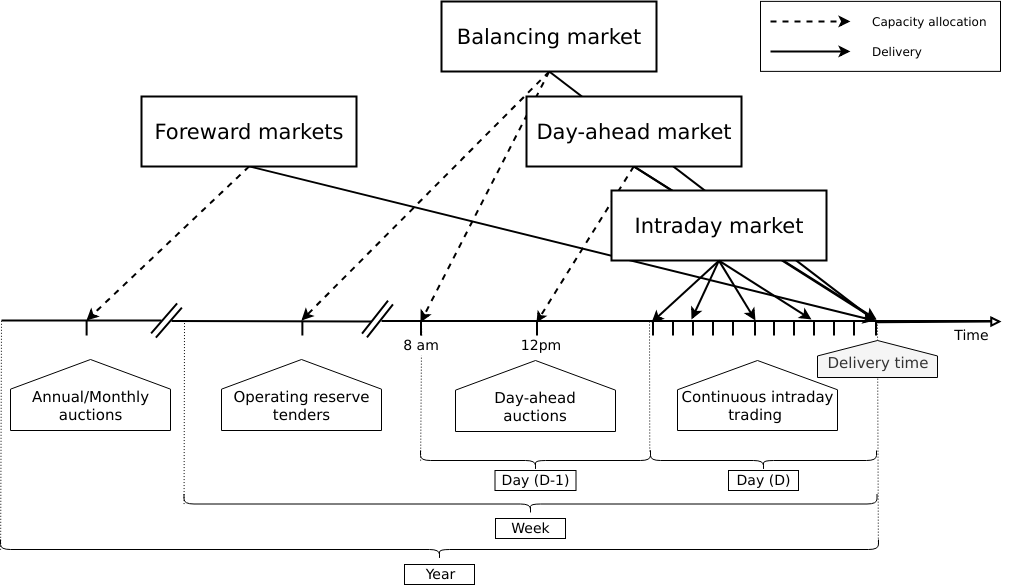
\includegraphics[width=\linewidth]{fig/electricity-markets.png}
\caption[Electricity Market Design]{Interaction between electricity markets in relation to capacity allocation \label{fig-electricity-markets}}
\end{figure}
\subsection{Electricity Market Theory}
\label{sec:orgbc5a1aa}
\subsubsection{Balancing Market \label{sec-balancing-market}}
\label{sec:org97c1025}
The balancing market is a tool to balance frequency deviations in the power
grid. It offers auctions for primary control reserve, secondary control reserve
as well as tertiary control reserve (minute reserve), which primarily differ in
the required ramp-up times of the participants. As depicted in Figure
\ref{fig-electricity-markets}, the balancing market can be seen as the last link
in a chain of electricity markets \cite{veen16_elect_balan_market}. \red{Explain!}
In this study, we will look at the German Control Reserve Market (GCRM), one of
the largest frequency regulation markets in the world. However, the presented
concepts can be easily transferred to other balancing markets in unbundled
energy systems, since the market design is similar
\cite{brandt17_evaluat_busin_model_vehic_grid_integ}. Transmission Systems
Operators (TSO) procure their required control reserve via tender auctions at
the GCRM. The market conducts daily auctions for the three types of control
reserve. This thesis focuses on the secondary operating reserve auction, in
which participants must be able to supply or absorb a minimum of 1MW of power
over a 4-hour interval with a reaction time of 30 seconds.\footnote{See \url{https://regelleistung.net}, accessed on 15\textsuperscript{th} February
2019, for further information on the market design and historical data.} Since EV
batteries can absorb energy almost instantly, when they are connected to a
charging station, they are suitable to provide such balancing services.
Operating reserve providers have to be qualified by the TSO to participate in
the market and are able to reliably provide the committed capacity. Although EV
fleets are currently not qualified by the GCRM to be used as operating reserve,
they could theoretically handle the minimum capacity requirements. Around 220
EVs would need to simultaneously charge at standard 4.6kW charging stations to
provide 1MW of downward regulating capacity.

Up until 28\textsuperscript{th} July 2018, auctions were held weekly, with two different
segments each week (peak hours/non-peak hours). Afterwards, the auction
mechanism changed to \emph{daily} auctions of six four-hour segments of positive and
negative control reserve.\footnote{\url{https://www.bundesnetzagentur.de/SharedDocs/Pressemitteilungen/DE/2017/28062017\_Regelenergie.html},
accessed 18\textsuperscript{th} February, 2019} Shorter auction cycles facilitate the
integration of renewable energy generators into the secondary control reserve
market, as they are dependent on accurate (short-term) capacity forecasts.

Positive control reserve is energy that is supplied to the grid, when the grid
frequency falls below 50Hz. It can be provided by increasing the electricity
generation or by reducing the grid load (i.e., electricity consumption). On the
contrary, negative control reserve is required when the grid frequency rises
above 50Hz and can be provided by adding grid load or reducing electricity
generation. Since we do not consider V2G in this thesis, the EV fleets in our
model are only able provide \emph{negative control reserve}, which we will refer to
as \emph{control reserve} until the end of the thesis. Market participants submit
bids in the following form to the market: \((\Pb{}, \cp{}, \ep{})\), where \(\Pb{}\)
is the amount of electrical power that can be supplied on demand in kW, \(\cp{}\) is
the capacity price for keeping the power available in \(\emw\) and
\(\ep{}\) is the energy price for delivered energy in \(\emwh\). The TSO
determines the target quantity of energy to acquire per timeslot, it usually
acquires much higher regulation capacity to minimize risks and activates the
capacity on demand. The TSO accepts the bids based on the capacity price in a
merit order. Providers, whose bids were accepted, instantly get compensated for
the provided capacity: \(R^c = \cp{} \times \Pb{}\). At the time regulation
capacity is needed, usually a day to a week later, the TSO activates the
capacity according to a merit order of the ascending \emph{energy prices} \(\ep{}\).
Hence, providers are also compensated according to the actual energy \(\Eb{}\)
they supplied or consumed: \(R^e = \ep{} \times \Eb{}\). Since provider get paid
according to their submitted price \(\ep{}\), instead of a market clearing price,
this type of auction is called \emph{pay-as-bid} auction.
\subsubsection{Spot Market \label{sec-spot-market}}
\label{sec:org97ceffa}
As mentioned in the previous chapter, the equilibrium of electricity supply and
demand is ensured through a sequence of interdependent wholesale markets
\cite{pape16_are_fundam_enoug}. Next to the balancing market at the end of the
sequence, mainly two different types of spot markets exist, the day-ahead market
and the intraday market. In this research, we consider the European Power
Exchange (EPEX Spot) as it is the largest electricity market in Europe, with a
total trading volume of approximately 567TWh in 2018\footnote{\url{https://www.epexspot.com/en/press-media/press/details/press/Traded\_volumes\_soar\_to\_an\_all-time\_high\_in\_2018},
accessed 19\textsuperscript{th} February, 2019\label{org04a7ba6}}, but most electronic
spot markets in western economies work with similar market mechanisms.

In Germany, the most important spot market is the day-ahead market with a
trading volume of over 234TWh in 2018\textsuperscript{\ref{org04a7ba6}}. Participants place asks and bids
for hourly contracts of the following day on the \emph{EPEX Spot Day-ahead Auction}
market until the market closes at 12pm on the day before delivery (see Figure
\ref{fig-electricity-markets}). The day-ahead market plays an essential role in
integrating volatile renewable energy sources (RES) into the power system
\cite{pape16_are_fundam_enoug}. Generators forecast the expected generation
capacity for the next day and sell those quantities on the market
\cite{karanfil17_role_contin_intrad_elect_market}. After the market closes, the
participants have the opportunity to trade the difference between the day-ahead
forecast and the more accurate intraday forecast on the intraday market
\cite{kiesel17_econom_analy_intrad_elect_prices}. In this way, RES generators can
cost effectively self-balance their portfolios, instead of relying on balancing
services provided by the TSO, which imposes high imbalance costs on participants
\cite{pape16_are_fundam_enoug}.

On the \emph{EPEX Spot Intraday Continuous} market, electricity products are traded
up until 5 minutes before physical delivery. Hourly contracts, as well as
15-minute and block contracts, can be traded. In contrast to the day-ahead
auction, the intraday market is a continuous order-driven market. Participants
can submit limit orders at any time during the trading window and equally change
or withdraw the order at any time before the order is accepted. Limit orders are
specified as price-quantity pairs: \((\Pi{}, \up{})\), where \(\Pi{}\) is the
traded amount of electrical power in kW and \(\up{}\) is the price for the delivered
energy unit (hour/quarter/block) in \(\emwh\). When an order to buy
(bid) matches an order to sell (ask), the trade immediately gets executed. The
order book is visible to all participants, hence it is known which unmatched
orders exist at the time of interest. The intraday market has a trading volume
of 82TWh, which is considerably smaller than day-ahead market's volume. Despite
that, the intraday market plays a vital role to the stability of the grid. All
executed trades on the intraday market potentially reduce the activation of
control reserve through the TSO.

Purchasing electricity on the continuous intraday market is attractive for EV
fleets with uncertain mobility demand. Due to the intradays market's short time
before delivery, EV fleet operators can rely on highly accurate forecasts of
available battery capacity to charge, before submitting an order to buy. In this
way, they can reliably charge at a potentially lower price at the intraday
market than the regular industry tariff. In an integrated bidding strategy, EV
fleet operators can, similarly to RES generators, balance out forecast errors of
available battery capacity on the intraday market. Trades on the intraday market
can complement bids that have been committed to other markets earlier (e.g., to
the secondary operating reserve market).
\subsection{EV Fleet Control in the Smart Grid}
\label{sec:orgbf637c2}
The increasing penetration of EVs has a substantial effect on electricity
consumption patterns. During charging periods, power flows and grid losses
increase considerably and challenge the grid. Operators have to reinforce the
grid to ensure that transformers and substations do not overload
\cite{sioshansi12_impac_elect_tarif_plug_in,lopes11_integ_elect_vehic_elect_power_system}.
Loading multiple EVs in the same neighborhood, or worse, whole EV fleets at
once, stress the grid. In these cases, even brown- or blackouts can occur.
\cite{kim12_carbit}. Despite these challenges, it is possible to support the
physical reinforcement by adopting smart charging strategies. In smart charging,
EVs get charged when the grid is less congested to ensure grid stability. Smart
charging reduces peaks in electricity demand, called \emph{Peak Cutting}, and
complement the grid in times of low demand, called \emph{Valley Filling}. Smart
charging has been researched thoroughly in the IS literature, in the following
we will outline some of the most important contributions.


\textcite{valogianni14_effec_manag_elect_vehic_storag} found that using
intelligent agents to schedule EV charging substantially reshapes the energy
demand and reduces peak demand without violating individual household
preferences. Moreover, they showed that the proposed smart charging behavior
reduces average energy prices and thus benefit households economically. In
another study, \textcite{kara15_estim_benef_elect_vehic_smart} investigated the
effect of smart charging on public charging stations in California. Controlling
for arrival and departure times, the authors presented beneficial results for
the distribution system operator (DSO) and the owners of EVs. Their approach
resulted in a price reduction in energy bills and a peak load reduction. An
extension of the smart charging concept is Vehicle-to-Grid (V2G). When equipped
with V2G devices, EVs can discharge their batteries back into the grid. Existing
research has focused on this technology in respect to grid stabilization effects
and arbitrage possibilities. For instance,
\textcite{schill11_elect_vehic_imper_elect_market} showed that the usage of EVs
can decrease average consumer electricity prices. Excess EV battery capacity can
be used to charge in off-peak hours and discharge in peak hours, when the prices
are higher. These arbitrage possibilities reverse welfare effects of generators
and increase the overall welfare and consumer surplus.
\textcite{tomic07_using_fleet_elect_drive_vehic_grid_suppor} found that the
arbitrage opportunities are especially prominent when a high variability in
electricity prices on the target electricity market exists. The authors stated
that short intervals between the contract of sale and the physical delivery of
electricity increase arbitrage benefits. Consequently, ancillary service
markets, like frequency control and operating reserve markets, are attractive
for smart charging.

\textcite{peterson10_econom_using_plug_in_hybrid} investigated energy arbitrage
profitability with V2G in the light of battery depreciation effects in the US.
The results of their study indicate that large-scale use of EV batteries for
grid storage does not yield enough monetary benefits to incentivize EV owners to
participate in V2G activities. Considering battery depreciation cost, the
authors arrived at an annual profit of only 6\$ - 72\$ per EV.
\textcite{brandt17_evaluat_busin_model_vehic_grid_integ} evaluated a business
model for parking garage operators operating on the German frequency regulation
market. When taking infrastructure costs and battery depreciation costs into
account, they conclude that the proposed vehicle-grid integration is not
profitable. Even with idealized assumptions about EV adoption rates in Germany
and altered auction mechanisms, the authors arrived at negative profits.
\textcite{kahlen17_fleet} used EV fleets to offer balancing services to the grid.
Evaluating the impact of V2G in their model, the authors conclude that V2G would
only be profitable if reserve power prices were twice as high. Considering the
results from the studies mentioned above, our research does not include V2G,
since only marginal profits are expected.

In order to maximize profits, it is essential for market participants to develop
successful bidding strategies. Several authors have investigated bidding
strategies to jointly participate in multiple markets
\cite{mashhour11_biddin_strat_virtual_power_plant_2,he16_optim_biddin_strat_batter_storag}.
\textcite{mashhour11_biddin_strat_virtual_power_plant_2} used stationary battery
storage to participate in the spinning reserve market and the day-ahead market
at the same time. The authors developed a non-equilibrium model, which solves
the presented mixed-integer program with genetic programming. Contrarily,
we use a model-free RL agent that learns an optimal policy (i.e., a trading
strategy) from actions it takes in the environment (i.e., bidding on electricity
markets). Using a model-free approach is especially beneficial for us, since
additional unknown variables and constraints (i.e., customer mobility demand)
complicate the formulation of a mathematical model.

\textcite{he16_optim_biddin_strat_batter_storag} conducted similar research to
\textcite{mashhour11_biddin_strat_virtual_power_plant_2}. The authors additionally
incorporated battery life cycle in their profit maximization model, which proved
to be a decisive factor. In contrast to the authors, we jointly participated in
the secondary operating reserve and spot market with the \emph{non-stationary}
storage of EV batteries. Because shared EVs have to satisfy mobility demand,
they have to be charged in any case, which allows us to safely exclude battery
depreciation from our model. Further, we chose the intraday market over the
day-ahead market, as it has the lowest reaction time among the spot markets, and
thus potentially offers higher profits
\cite{tomic07_using_fleet_elect_drive_vehic_grid_suppor}.

Previous studies often assume that car owners or households can directly trade
on electricity markets. In reality, this is not possible due to the minimum
capacity requirements of the markets, requirements that single EVs do not meet.
For example, the German Control Reserve Market (GCRM) has a minimum trading
capacity of 1MW to 5MW, depending on the specific market. In order to reach the
minimum capacity, over 200 EVs would need to be connected to the grid via a
standard 4.6kW charging station at the same time. \textcite{ketter13_power_tac}
introduced the notion of electricity brokers, aggregators that act on behalf of
a group of individuals or households to participate in electricity markets.
\textcite{brandt17_evaluat_busin_model_vehic_grid_integ} and
\textcite{kahlen14_balan_with_elect_vehic} successfully showed that electricity
brokers can overcome the capacity issues by aggregating EV batteries. In
addition to electricity brokers, we apply the concept of Virtual Power Plants
(VPPs). VPPs are flexible portfolios of distributed energy resources, which are
presented with a single load profile to the system operator, making them
eligible for market participation and ancillary service provisioning
\cite{pudjianto07_virtual_power_plant_system_integ}. Hence, VPPs allow providing
regulation capacity to the market without knowing which exact sources provide
the promised capacity until the delivery time \cite{kahlen17_fleet}. This concept
is specially useful when dealing with EV fleets: VPPs enable carsharing
providers to issue bids and asks based on an estimate of available fleet
capacity, without knowing beforehand which exact EVs will provide the capacity
at the time of delivery. Based on the battery charge and the availability of
EVs, an intelligent agent decides in real-time which vehicles provide the
capacity.

Centrally managed EV fleets make it possible for carsharing providers to use the
presented concepts as a viable business extension. Free float carsharing is a
popular mobility concept that allows cars to be picked up and parked everywhere,
and the customers are billed is by the minute. Free float carsharing offers
flexibility to its users, saves resources, and reduces carbon emissions
\cite{firnkorn15_free_float_elect_carsh_fleet_smart_cities}. Most previous studies
concerned with the usage of EVs for electricity trading, assumed that trips are
fixed and known in advance, e.g., in
\textcite{tomic07_using_fleet_elect_drive_vehic_grid_suppor}. The free float
concept adds uncertainty and nondeterministic behavior, which make predictions
about future rentals a complex issue.

\textcite{kahlen17_fleet} showed that it is possible to use free float carsharing
fleets as VPPs to profitably offer balancing services to the grid. In their
study, the authors compared cases from three different cities across Europe and
the US. They used an event-based simulation, bootstrapped with real-world
carsharing and secondary operating reserve market data from the respective
cities. A central dilemma within their research was to decide whether an EV
should be committed to a VPP or free for rent. Since rental profits are
considerably higher than profits from electricity trading, it is crucial not to
allocate an EV to a VPP when it could have been rented out otherwise. To deal
with the asymmetric payoff, \citeauthor{kahlen17_fleet} used stratified sampling
in their classifier. This method gives rental misclassifications higher weights,
reducing the likelihood of EVs to participate in VPP activities. The authors
used a Random Forest regression model to predict the available balancing
capacity on an aggregated fleet level. Only at the delivery time, the agent
decides which individual EVs provide the regulation capacity. This heuristic is
based on the likelihood that the vehicle is rented out and on its expected
rental benefits.

In a similar study, the authors showed that carsharing companies can participate
in day-ahead markets for arbitrage purposes
\cite{kahlen18_elect_vehic_virtual_power_plant_dilem}. In the paper, the authors
used a sinusoidal time-series model to predict the available trading capacity.
Another central problem for carsharing providers is that committed trades, which
can not be fulfilled, result in substantial penalties from the system operator
or electricity exchange. In other words, fleet operators have to avoid buying
any amount of electricity, which they can't be sure to charge with available EVs
at the delivery time. To address this issue, the authors developed a mean
asymmetric weighted objective function. They used it for their time-series based
prediction model, to penalize committing an EV to VPP when it would have been
rented out otherwise. Because of the two issues mentioned above,
\textcite{kahlen18_elect_vehic_virtual_power_plant_dilem} could only make very
conservative estimations and commitments of overall available trading capacity,
resulting in a high amount of missed profits. This effect is especially
prominent when participating in the secondary operating reserve market, since
commitments have to be made one week in advance when mobility demands are still
uncertain. \textcite{kahlen17_fleet} stated that in 42\% to 80\% of the cases, EVs
are not committed to a VPP when it would have been profitable to do so.

This thesis proposes a solution in which the EV fleet participates in the
balancing market and intraday market simultaneously. With this approach, we
align the potentially higher profits on the balancing markets, with more
accurate capacity predictions for intraday markets
\cite{tomic07_using_fleet_elect_drive_vehic_grid_suppor}. This research followed
\textcite{kahlen17_fleet}, who proposed to work on a combination of multiple
markets in the future.

\subsection{Reinforcement Learning Controlled EV Charging}
\label{sec:org5307ed1}

Previous research shows that intelligent agents equipped with Reinforcement
Learning (RL) methods can successfully take action in the smart grid. The
following chapter outlines different research approaches of RL in the domain of
smart grids. For a more thorough description, mathematical formulations and
common issues, of RL refer to Chapter \ref{sec-reinforcement-learning}.

\textcite{reddy11_learn_behav_multip_auton_agent,reddy11_strat} used autonomous
broker agents to buy and sell electricity from DER on a proposed \emph{Tariff
Market}. The agents use Markov Decision Processes (MDPs) and RL to learn pricing
strategies to profitably participate in the Tariff Market. To control for a
large number of possible states in the domain, the authors used \emph{Q-Learning}
with derived state space features. Based on descriptive statistics, they defined
derived price and market participant features. By engaging with its environment,
the agent learns an optional sequence of actions (policy) based on the state of
the agent. \textcite{peters13_reinf_learn_approac_to_auton} built on that work and
further enhanced the method by using function approximation. Function
approximation allows to efficiently learn strategies over large state spaces, by
deriving a function that describes the states instead of defining discrete
states. By using this technique, the agent can adapt to arbitrary economic
signals from its environment, resulting in better performance than previous
approaches. Moreover, the authors applied feature selection and regularization
methods to explore the agent's adaption to the environment. These methods are
particularly beneficial in smart markets because market design, structures, and
conditions might change in the future. Hence, intelligent agents should be able
to adapt to it \cite{peters13_reinf_learn_approac_to_auton}.

\textcite{vandael15_reinf_learn_heuris_ev_fleet} facilitated learned EV fleet
charging behavior to optimally purchase electricity on the day-ahead market.
Similarly to \textcite{kahlen18_elect_vehic_virtual_power_plant_dilem}, the
problem is framed from the viewpoint of an aggregator that tries to define a
cost-effective day-ahead charging plan in the absence of knowing EV charging
parameters, such as departure time. A crucial point of the study is weighting
low charging prices against costs that have to be paid when an excessive or
insufficient amount of electricity is bought from the market (imbalance costs).
Contrarily, \textcite{kahlen18_elect_vehic_virtual_power_plant_dilem} did not
consider imbalance cost in their model and avoid them by sacrificing customer
mobility in order to balance the market (i.e., not showing the EV available for
rent, when it is providing balancing capacity).
\textcite{vandael15_reinf_learn_heuris_ev_fleet} used a \emph{fitted Q Iteration} to
control for continuous variables in their state and action space. In order to
achieve fast convergence, they additionally optimized the \emph{temperature step}
parameter of the Boltzmann exploration probability.

\textcite{dusparic13_multi} proposed a multi-agent approach for residential demand
response. The authors investigated a setting in which 9  EVs were connected to
the same transformer. The RL agents learned to charge at minimal costs, without
overloading the transformer. \textcite{dusparic13_multi} utilized \emph{W-Learning} to
simultaneously learn multiple policies (i.e., objectives such as ensuring
minimum battery charged or ensuring charging at low costs).
\textcite{taylor14_accel_learn_trans_learn} extended this research by employing
Transfer Learning and \emph{Distributed W-Learning} to achieve communication between
the learning processes of the agents in a multi-objective, multi-agent setting.
\textcite{dauer13_market_based_ev_charg_coord} proposed a market-based EV fleet
charging solution. The authors introduced a double-auction call market where
agents trade the available transformer capacity, complying with the minimum
required State of Charge (SoC). The participating EV agents autonomously learn
their bidding strategy with standard \emph{Q-Learning} and discrete state and action
spaces.

\textcite{di13_elect_vehic} presented a multi-agent solution to minimize charging
costs of EVs, a solution that requires neither prior knowledge of electricity
prices nor future price predictions. Similar to
\textcite{dauer13_market_based_ev_charg_coord}, the authors employed standard
\emph{Q-Learning} and the \(\epsilon\)-greedy approach for action selection.
\textcite{vaya14_optim} also proposed a multi-agent approach, in which the
individual EVs are agents that actively place bids in the spot market. Again,
the agents use \emph{Q-Learning}, with an \(\epsilon\)-greedy policy to learn their
optimal bidding strategy. The latter relies on the agents willingness-to-pay
which depends on the urgency to charge. State variables, such as SoC, time of
departure and price development on the market, determine the urgency to charge.
The authors compared this approach with a centralized aggregator-based approach
that they developed in another paper \cite{vaya15_optim_biddin_strat_plug_in}.
Compared to the centralized approach, in which the aggregator manages charging
and places bids for the whole fleet, the multi-agent approach causes slightly
higher costs but solves scalability and privacy problems.

\textcite{shi11_real} consider a V2G control problem, while assuming real-time
pricing. The authors proposed an online learning algorithm which they modeled as
a discrete-time MDP and solved through \emph{Q-Learning}. The algorithm controls the
V2G actions of the EV and can react to real-time price signals of the market. In
this single-agent approach, the action space compromises only charging,
discharging and regulation actions. The limited action spaces makes it
relatively easy to learn an optimal policy.
\textcite{chis16_reinf_learn_based_plug_in} looked at reducing the costs of
charging for a single EV using known day-ahead prices and predicted next-day
prices. A Bayesian ANN was employed for prediction and \emph{fitted Q-Learning} was
used to learn daily charging levels. In their research, the authors used
function approximation and batch reinforcement learning, an offline, model-free
learning method. \textcite{ko18_mobil_aware_vehic_to_grid} proposed a centralized
controller for managing V2G activities in multiple microgrids. The proposed
method considers mobility and electricity demands of microgrids, as well as SoC
of the EVs. The authors formulated a MDP with discrete state and action spaces
and use standard \emph{Q-Learning} with \(\epsilon\)-greedy policy to derive an optimal
charging policy. The approach takes microgrid autonomy and electricity prices
into special consideration.

It should be noted that advanced RL methods and techniques are not the only
solutions for problems in the smart grid, often basic algorithms and heuristics
provide satisfactory results \cite{vazquez-canteli19_reinf_learn_deman_respon}.
Despite that, our paper considers RL as an optimal fit for the design of our
proposed intelligent agent. Given the ability to learn user behavior (e.g.,
mobility demand) and the flexibility to adapt to the environment (e.g.,
electricity prices), RL methods are a promising way of solving complex
challenges in smart grids.

\subsection{Reinforcement Learning Theory \label{sec-reinforcement-learning}}
\label{sec:org31df758}
The following chapter will give an overview of the most important Reinforcement
Learning (RL) concepts and will introduce the corresponding mathematical
formulations. If not noted otherwise, the notation, equations, and insights are
adopted from \cite{sutton18_reinf}, the de-facto reference book of RL research.

RL is an agent-based machine learning algorithm in which the agent learns to
perform an optimal set of actions through interaction with its environment. The
agents objective is to maximize the rewards it receives based on the actions it
takes. Immediate rewards have to be weighted against long-term cumulative
returns that also depend on the agent's future actions. The RL problem is
formalized as Markov Decision Processes (MDPs) which will be introduced in
Chapter \ref{sec-mdp}. A critical task of RL agents is to continuously estimate
the value of the environment's state. Values indicate the long-term desirability
of a state, that is the total amount of reward the agent can expect to
accumulate over the future, following a learned set of actions, called the
policy. Policies and values are covered in Chapter \ref{sec-policies}, whereas the
core mathematical foundations for evaluating policies and updating value
functions are introduced in Chapter \ref{sec-bellman}. When the model of the
environment is fully known, the learning problem is reduced to a planning
problem (Chapter \ref{sec-dp}) in which optimal policies can be computed with
iterative approaches. Model-free RL approaches can be applied when rewards and
state transitions are unknown, and the agent's behavior has to be learned from
experience (Chapter \ref{sec-td-learning}). The last two chapter cover methods
that solve the RL problem more efficiently, tackle new challenges and are widely
used in practice and research.

\subsubsection{Markov Decision Processes \label{sec-mdp}}
\label{sec:orgb68c85d}
Markov Decision Processes (MDPs) are a classical formulation of sequential
decision making and an idealized mathematical formulation of the RL problem. MDPs
allow to derive exact theoretical statements about the learning problem and
possible solutions. Figure
\ref{agent-environment-interaction} depicts the \emph{agent-environment interaction}.
\begin{figure}[htbp]
\centering
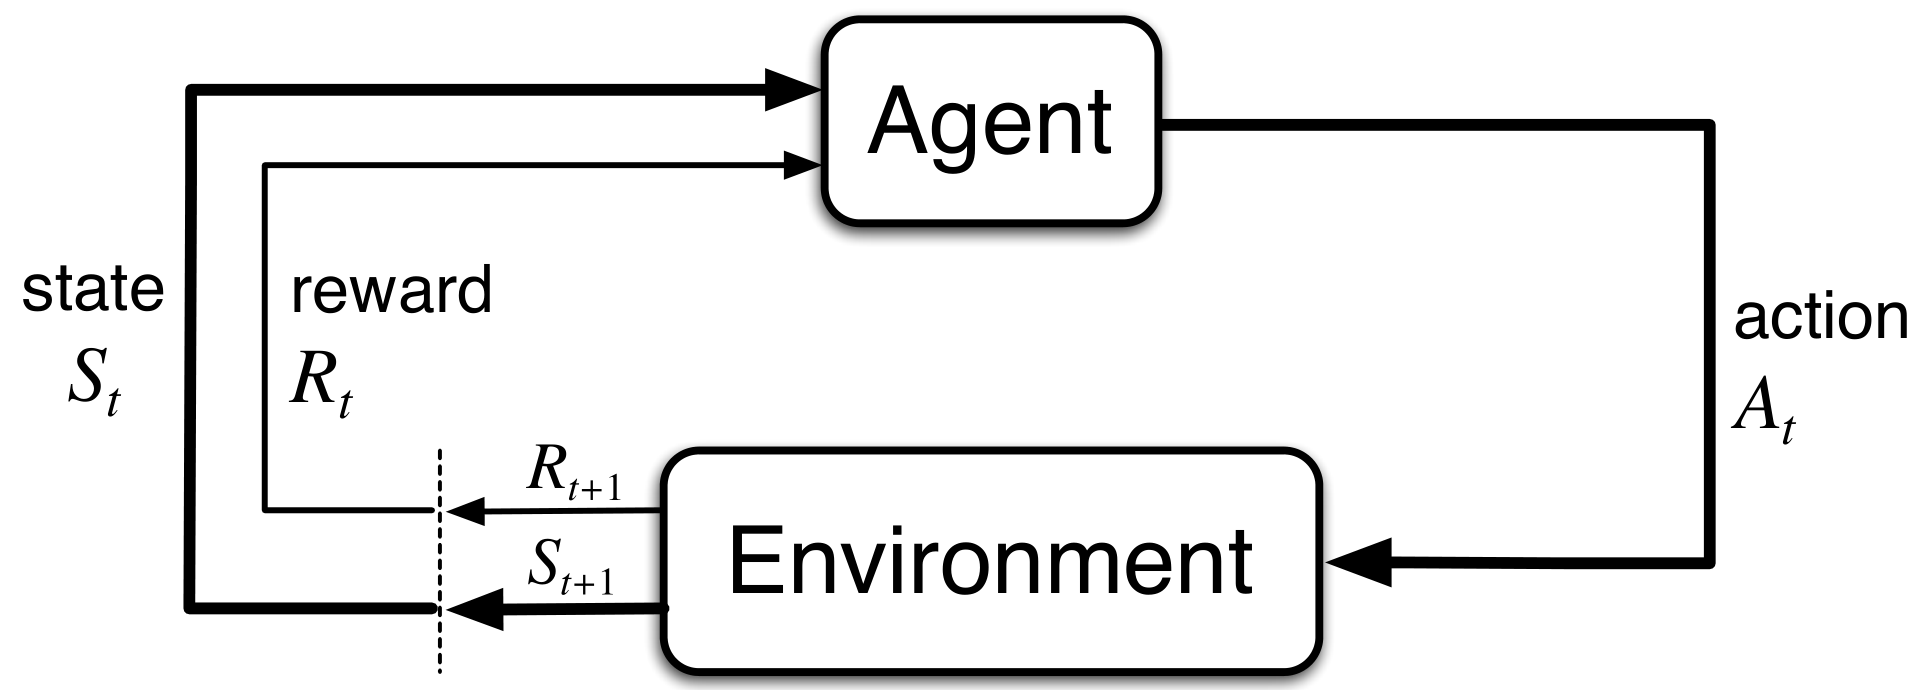
\includegraphics[width=0.85\linewidth]{fig/mdp-interaction.png}
\caption[Markov Decision Process]{The agent-environment interaction in a Markov decision process \cite{sutton18_reinf} \protect\footnotemark \label{agent-environment-interaction}}
\end{figure}
\footnotetext{\textbf{Figure 3.1} from "Reinforcement Learning: An Introduction" by Richard S. Sutton and Andew G. Barto is licencsed under CC BY-NC-ND 2.0 (https://creativecommons.org/licenses/by-nc-nd/2.0/)}

In RL the agent and the environment continuously interact with each other. The
agent takes actions that influence the environment, which in return presents
rewards to the agent. The agent's goal is to maximize rewards over time, trough
an optimal choice of actions. In each discrete timestep \(t\!=\!0,1,2,...,T\) the
RL agent interacts with the environment, which is perceived by the agent as a
representation, called \emph{state}, \(S_t \in \S\). Based on the state, the agents
selects an \emph{action}, \(A_t\in\A\), and receives a numerical \emph{reward} signal,
\(R_{t+1}\in\R\subset\Re\), in the next timestep. Actions influence immediate
rewards and successive states, and consequently also influence future rewards.
The agent has to continuously make a trade-off between immediate rewards and
delayed rewards to achieve its long-term goal.

The \emph{dynamics} of a MDP are defined by the probability that a state \(s'\in \S\)
and a reward \(r\in\R\) occurs, given the preceding state \(s\in\S\) and action
\(a\in\A\). In \emph{finite} MDPs, the random variables \(R_t\) and \(S_t\) have
well-defined probability density functions (PDF), which are solely dependent on
the previous state and action. Consequently, it is possible to define (\(\defeq\))
the \emph{dynamics} of the MDP as follows:
\begin{equation}
    p(s',r|s,a) \defeq \Pr{S_t=s',R_t=r|S_{t-1}=s,A_t=a},
\end{equation}
for all \(s',s\!\in\!\S\), \(r\!\in\!\R\) and \(a\!\in\!\A\). Note that each possible
value of the state \(\S_t\) depends only on the immediately preceding state
\(\S_{t-1}\). When a state includes all information of \emph{all} previous states, the
state possesses the so-called \emph{Markov property}. If not noted otherwise, the
Markov property is assumed throughout the whole chapter. The dynamics function
allows computing the \emph{state-transition probabilities}, another important
characteristic of an MDP, as follows:
\begin{equation}
    p(s'|s,a) \defeq \Pr{S_t\!=\!s'|S_{t-1}\!=\!s,A_t\!=\!a} = \sum_{r\in\R}{p(s', r|s, a)},
\end{equation}
for \(s',s\!\in\!\S\), \(r\!\in\!\R\) and \(a\!\in\!\A\).

The use of a \emph{reward signal} \(R_t\) to formalize the agent's goal is a unique
characteristic of RL. Each timestep the agent receives the rewards as a scalar
value \(\R_t\in\Re\). The sole purpose of the RL agent is to maximize the
long-term cumulative reward (as opposed to the immediate reward). The long-term
cumulative reward can also be expressed as the \emph{expected return} \(G_t\):
\begin{equation} \label{eq-expected-return}
\begin{split}
    G_t &\defeq R_{t+1} + \gamma R_{t+2} + \gamma R_{t+3} + \cdots \\
    &= \sum_{k=0}^{\infty}{\gamma^k R_{t+k+1}} \\
    &= R_{t+1} + \gamma G_{t+1},
\end{split}
\end{equation}
where \(\gamma\), \(0\leq\gamma\leq 1\), is the \emph{discount rate} parameter. The
discount rate determines how "myopic" the agent is. If \(\gamma\) approaches 0,
the agent is more concerned with maximizing immediate rewards. On the contrary,
when \(\gamma\!=\! 1\), the agent takes future rewards strongly into account, the
agent is "farsighted".

\subsubsection{Policies and Value Functions \label{sec-policies}}
\label{sec:org01fd91a}
An essential task of almost every RL agent is estimating \emph{value functions}.
These functions describe how "good" it is to be in a given state, or how "good"
it is to perform an action in a given state. More formally, they take a state
\(s\) or a state-action pair \(s,a\) as input and give the expected return \(G_t\) as
output. The expected return is dependent on the actions the agent will take in
the future. Consequently, value functions are formulated with respect to a
\emph{policy} \(\pi\). A policy is a mapping of states to actions; it describes the
probability that an agent performs a certain action, based on the current state.
More formally, the policy is defined as
\(\pi(a|s)\defeq\Pr{A_t\!=\!a|S_t\!=\!s}\), a PDF of all \(a\!\in\!\A\) for each
\(s\!\in\!\S\). RL approaches mainly differ in how the policy is updated, based on
the agent's interaction with the environment.

In RL, value functions of states and value functions of state-action pairs are
used. The \emph{state-value function of policy} \(\pi\) is denoted as \(\vpi(s)\) and is
defined as the expected return when starting in \(s\) and following policy \(\pi\):
\begin{equation}
    \vpi(s) \defeq \EE{\pi}{G_t|S_t\!=\!s}, \text{ for all } s\in\S
\end{equation}
The \emph{action-value function of policy} \(\pi\) is denoted as \(\qpi(s,a)\) and is
defined as the expected return when starting in \(s\), taking action \(a\) and
following policy \(\pi\) afterwards:
\begin{equation}
    \qpi(s,a) \defeq \EE{\pi}{G_t|S_t\!=\!s, A_t\!=\!a}, \text{ for all } a\in\A, s\in\S
\end{equation}
The \emph{optimal policy} \(\pi_*\) has a greater (or equal) expected return than all
other policies. The \emph{optimal} state-value function and \emph{optimal} action-value
function are defined as follows:
\begin{equation}
    \vstar(s) \defeq \max_{\pi} \vpi(s), \text{ for all } s\in\S
\end{equation}
\begin{equation}
    \qstar(s,a) \defeq \max_{\pi} \qpi(s,a), \text{ for all } s\in\S, a\in\A
\end{equation}
The \emph{optimal} action-value function describes the expected return when taking
action \(a\) in state \(s\) following the optimal policy \(\pi_*\) afterwards.
Estimating \(\qstar\) to obtain an optimal policy is a substantial part of RL and
has been known as \emph{Q-learning} \cite{watkins92_q_learn}, which is described in
Chapter \ref{sec-td-learning}.

\subsubsection{Bellman Equations \label{sec-bellman}}
\label{sec:orgdb01ab2}
A central characteristic of value functions is the recursive relationship
between the values. Similar to Equation (\ref{eq-expected-return}), current values
are related to expected values of successive states. This relationship is
heavily used in RL and has been formulated as \emph{Bellman equations}
\cite{bellman57_dynam_progr}. The Bellman equation for \(\vpi(s)\) is defined as
follows:
\begin{equation} \label{eq-bellman}
\begin{split}
    \vpi(s) &\defeq \EE{\pi}{G_t|S_t=s} \\
    &= \EE{\pi}{R_{t+1}+\gamma G_{t+1}|S_t\!=\!s} \\
    &= \sum_{a}{\pi(a|s)}\sum_{s',r}{p(s',r|s,a)}\bigg[r+\gamma\vpi(s')\bigg],
\end{split}
\end{equation}
where \(a\!\in\!\A\), \(s,s'\!\in\!\S\), \(r\!\in\!\R\).
In other words, the value of a state equals the immediate reward plus the
expected value of all possible successor states, weighted by their probability
of occurring. \(\vpi(s)\) is the only solution to its Bellman equation. The
Bellman equation of the optimal value function \(v_*\) is called the \emph{Bellman
optimality equation}:
\begin{equation} \label{eq-bellman-optimality}
\begin{split}
    \vstar(s) &\defeq \max_{a\in\A(s)}q_{\pi_*}(s,a) \\
    &= \max_{a}\EE{\pi_*}{R_{t+1}+\gamma G_{t+1}|S_t\!=\!s, A_t\!=a} \\
    &= \max_{a}\EE{\pi_*}{R_{t+1}+\gamma \vstar(S_{t+1})|S_t\!=\!s, A_t\!=a} \\
    &= \max_{a}\sum_{s',r}{p(s',r|s,a)}\bigg[r+\gamma\vstar(s')\bigg]
\end{split}
\end{equation}
where \(a\!\in\!\A\), \(s,s'\!\in\!\S\), \(r\!\in\!\R\). In other words, the value of
a state under an optimal policy equals the expected return for the best action
from that state. Note that the Bellman optimality equation does not refer to a
specific policy, it has a unique solution independent from one. It can be seen
as an equation system, which can be solved when the dynamics of the environment
\(p\) are known. Similar Bellman equations to Equations (\ref{eq-bellman}) and
(\ref{eq-bellman-optimality}) can also be formed for \(\qpi(s,a)\) and
\(\qstar(s,a)\). Bellman equations form the basis for computing and approximating
value functions and were an important milestone in RL history. Most RL methods
are \emph{approximately} solving the Bellman optimality equation, by using
experienced state transitions instead of expected transition probabilities. The
most common methods will be explored in the following chapters.

\subsubsection{Dynamic Programming \label{sec-dp}}
\label{sec:org64cf274}
\emph{Dynamic Programming} (DP) is a method to compute optimal policies, the primary
goal of every RL method. DP makes use of value functions to facilitate the
search for good policies. Once an optimal value function, (i.e., one that
satisfies the Bellman optimality equation) is found, optimal policies can be
easily obtained. Despite the limited utility of DP in real-world settings, it
provides the theoretical foundation for all RL methods. In fact, all of the RL
methods try to achieve the same goal, but without the assumption of a perfect
model of the environment and less computational effort. Because DP assumes full
knowledge of the environment, it is known as \emph{planning}, in which optimal
solutions are \emph{computed}. In \emph{control} problems (Chapter \ref{sec-td-learning}),
optimal solutions are \emph{learned} from an unknown environment.

The two most popular DP algorithms that compute optimal policies are called
\emph{policy iteration} and \emph{value iteration}. These methods perform "sweeps" through
the whole state set and update the estimated value of each state via an
\emph{expected update} operation. In policy iteration, a value function for a given
policy \(\vpi\) needs to be computed first, a step called \emph{policy evaluation}. A
sequence of approximated value functions \(\{v_k\}\) are updated using the Bellman
equation for \(\vpi\) (Eq. \ref{eq-bellman}) until convergence to \(\vpi\) is
achieved. After computing the value function for a given policy, it is possible
to modify the policy and see if the value \(\vpi(s)\) for a given state increases
(\emph{policy improvement}). A way of doing this, is evaluating the action-value
function \(\qpi(s,a)\) by \emph{greedily} taking the best short-term action \(a\!\in\!A\)
at a given timestep. Alternating between these two steps monotonically improves
the policies and the value functions until they converge to the optimum. This
algorithm is called \emph{policy iteration}:
\begin{equation}
    \pi_0 \xrightarrow{\text{ E }} v_{\pi_0} \xrightarrow{\text{ I }}
    \pi_1 \xrightarrow{\text{ E }} v_{\pi_1} \xrightarrow{\text{ I }}
    \pi_2 \xrightarrow{\text{ E }} \hdots \xrightarrow{\text{ I }}
    \pi_* \xrightarrow{\text{ E }} \vstar,
\end{equation}
where \(\xrightarrow{\text{ E }}\) denotes a policy evaluation step,
\(\xrightarrow{\text{ I }}\) denotes a policy improvement step. \(\pi_*\) and
\(\vstar\) are the optimal policy and optimal value function, respectively. Note
that in each iteration of the policy iteration algorithm, a policy evaluation
has to be performed, which requires multiple sweeps through the state space. In
\emph{value iteration}, the policy evaluation step is stopped after one sweep. In
this case, the two previous steps can be combined into one single update step:
\begin{equation}
\begin{split}
    v_{k+1}(s) &\defeq \max_a \EE{}{R_{t+1}+\gamma \vstar(S_{t+1})|S_t\!=\!s, A_t\!=a} \\
    &= \max_{a}\sum_{s',r}{p(s',r|s,a)}\bigg[r+\gamma v_k(s')\bigg],
\end{split}
\end{equation}
where \(a\!\in\!\A\), \(s,s'\!\in\!\S\), \(r\!\in\!\R\). It can be shown, that for any
given \(v_0\), the sequence \({v_k}\) converges to the optimal value function
\({\vstar}\). In value iteration, the Bellman optimality equation
(\ref{eq-bellman-optimality}) is simply turned into an update rule. Both of the
algorithms can be effectively used to compute optimal values and value function
in finite MDPs with a perfect model of the environment.

\subsubsection{Temporal-Difference Learning \label{sec-td-learning}}
\label{sec:org282922f}
The previous chapter dealt with solving a \emph{planning} problem, that is computing
an optimal solution (i.e., an optimal policy \(\pi_*\)) of an MDP when a perfect
model of the environment is known. In the following chapters, we will look at
\emph{model-free} prediction and \emph{model-free} control. As opposed to planning,
model-free methods learn from experience and require no prior knowledge of the
environment. Remarkably, these methods can still achieve optimal behavior.

The \emph{TD prediction problem} is concerned with estimating state-values \(\vpi\)
using past experiences of following a given policy \(\pi\). TD methods update an
estimate \(V\) of \(\vpi\) in every timestep. At time \(t\!+\!1\) they immediately
perform an update operation on \(V(S_t)\). Because of the step-by-step nature of
TD learning, it is categorized as \emph{online learning}. Also note that TD methods
perform update operations on value estimates based on other learned estimates, a
procedure called \emph{bootstrapping}. In simple TD prediction, the
value estimates \(V\) are updated as follows:
\begin{equation} \label{eq-td-prediction}
    V(S_t) \leftarrow V(S_t) + \alpha\big[R_{t+1}+\gamma V(S_{t+1}) - V(S_t)\big],
\end{equation}
where \(\alpha\) is a constant \emph{step-size} parameter and \(\gamma\) is the
\emph{discount rate}. Here, the update of the state-value is performed using the
observed reward \(R_{t+1}\) and the estimated value \(V(S_{t+1})\).

When a model is not available, it is useful to estimate \emph{action-values}, instead
of \emph{state-values}. If the environment is completely known, it is possible for
the agent to look one step ahead and select the best action. Without that
knowledge, the value of each action in a given state needs to be estimated. The
latter constitutes a problem, since not every \emph{state-action} pair will be
visited when the agent follows a deterministic policy. A deterministic policy
\(\pi(a|s)\) returns exactly one action given the current state, hence the agent
will only observe returns for one of the actions. In order to evaluate the value
function for all \emph{state-action} pairs \(\qpi\), continuous \emph{exploration} needs to
be ensured. In other words, the agent has to explore state-action pairs which
are seemingly disadvantageous given the current policy. This dilemma is also
known as the \emph{exploration-exploitation} trade-off. One way to achieve exploration
is using \emph{stochastic} policies for the action selection. Stochastic policies
have a non-zero probability of selecting each action in each state. A typical
stochastic policy is the \emph{\(\epsilon\)-greedy policy}, which selects the action with
the highest estimated value, except for a probability \(\epsilon\), it selects an
action at random.
\begin{figure}[htbp]
\centering
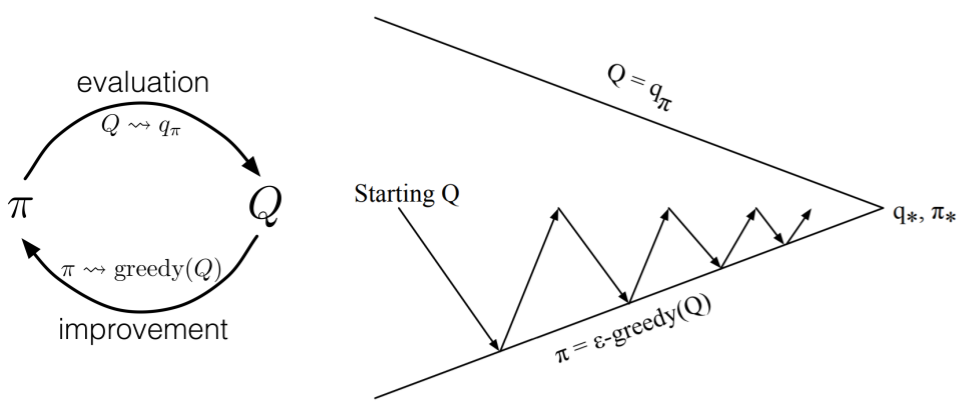
\includegraphics[width=0.85\linewidth]{fig/on-policy.png}
\caption[On-policy control with Sarsa]{On-policy control with Sarsa \cite{sutton18_reinf}. \protect\footnotemark \label{fig-sarsa}}
\end{figure}
\footnotetext{The in-text figure of \textbf{Chapter 5.3} from "Reinforcement Learning: An Introduction" by Richard S. Sutton and Andew G. Barto is licencsed under CC BY-NC-ND 2.0 (https://creativecommons.org/licenses/by-nc-nd/2.0/)}

There are two approaches to make use of stochastic policies to ensure all
actions are chosen infinitely often. On-policy methods improve the (stochastic)
decision policy, by continually estimating \(\qpi\) in regard to \(\pi\), while
simultaneously driving \(\pi\) towards \(\qpi\), e.g., with a \(\epsilon\)-greedy action
selection. Figure \ref{fig-sarsa} depicts this learning process. Off-policy
methods improve the deterministic decision policy, by using a second stochastic
policy to generate behavior. The first policy is becoming the optimal policy by
evaluating the exploratory behavior of the second policy. Off-policy approaches
are considered more powerful than on-policy approaches and have a variety of
additional use cases. On the other side, they often have a higher variance and
take more time to converge to an optimum.

A popular on-policy TD control method is Sarsa, developed by
\textcite{rummery94_q}. In the prediction step, the action-value function
\(\qpi(s,a)\) of all actions and states has to be estimated for the current
policy \(\pi\). The estimation can be done similar to TD prediction of state
values (Eq. \ref{eq-td-prediction}). Instead of considering state transitions,
state-action transitions are considered in this case. The update rule is
constructed as follows:
\begin{equation}
    Q(S_t, A_t) \leftarrow Q(S_t,A_t) + \alpha\big[R_{t+1}+\gamma Q(S_{t+1},A_{t+1}) - Q(S_t, A_t)\big]
\end{equation}
After every transition from a state \(S_t\), an update operation using the events
\((S_t, A_t, R_{t+1}, S_{t+1}, A_{t+1})\) is performed. This quintuple also
constituted the name Sarsa. The on-policy control step of the algorithm is
straightforward, and uses a \(\epsilon\)-greedy policy improvement, as described in
the previous paragraph. It has been shown that Sarsa converges to the optimal
policy \(\pi_*\) under the assumption of infinite visits to all state-action
pairs.

A breakthrough in RL has been achieved when \textcite{watkins92_q_learn} developed
the \emph{off-policy} TD control algorithm, called Q-learning. The update rule is
defined as follows:
\begin{equation}
    Q(S_t, A_t) \leftarrow Q(S_t,A_t) + \alpha\big[R_{t+1}+\gamma\max_a Q(S_{t+1},a) - Q(S_t, A_t)\big]
\end{equation}
Here, the estimated action-values \(Q\) are updated towards the highest estimated
action-value of the next time step. In this way, \(Q\) directly approximates the
optimal action-value function \(q_*\), independently of the policy the agent
follows. Due to this simplification, Q-learning is a widely used model-free
method, and its convergence can be proved easily \cite{watkins89_learn_from_delay_rewar}.

This chapter covered the most important RL methods. They work online, learn from
experience, and can be easily applied to real-world problems with low
computational effort. Moreover, the mathematical complexity of the presented
approaches is limited, and they can be easily implemented into computer
programs. Temporal-Difference learning is a \emph{tabular} method, in which Q-values
are stored and updated in a lookup table. If the state and action spaces are
continuous or the number of states and actions is very large, a table
representation is computational infeasible and the speed of convergence is
drastically reduced. In this case, a \emph{function approximator} can replace the
lookup table. The next chapter will briefly cover function approximation, as
well as other advancements in RL.
\subsubsection{Approximation Methods \label{sec-rl-fa}}
\label{sec:org0337252}
Up to this point, only tabular RL methods have been covered, which form the
theoretical foundation of RL in general. But in many real-world use cases, the
state space is enormous and it is improbable to find an optimal value function
with tabular methods. Not only is it a problem to store such a large table in
the memory, but also would it take an almost infinite amount of time to fill
every entry with meaningful results. Contrarily, \emph{function approximation} tries
to find a function that approximates the optimal value function as closely as
possible, with limited computational resources. The experience with a small
subset of visited states is generalized to approximate values of the whole state
set. Function approximation has been widely studied in supervised machine
learning: Gradient methods, as well as linear and non-linear models have shown
good results for RL.

The approximated value of a state \(s\) is denoted as the parameterized
functional form \(\hat v(s,\w)\!\approx\!\vpi(s)\), given a weight vector
\(\w\!\in\!\Re^d\). Function approximation methods are approximating \(\vpi\) by
learning (i.e., adjusting) the weight vector \(\w\) from the experience of following
the policy \(\pi\). By assumption, the dimensionality \(d\) of \(\w\) is much lower than
the number of states, which is the reason for the desired generalization effect:
Adjusting one weight affects the values of many states. However, optimizing
an estimate for one state negatively affects the accuracy of the estimates for
other states. This effect motivates the specification of a state distribution
\(\mu(s)\), which represents the importance of the prediction error for each state.
In on-policy prediction, \(\mu(s)\) is often selected to be proportion of time spend
in each state \(s\). The prediction error of a state is defined as the squared
difference between the predicted (i.e., approximated) value \(\hat v(s,\w)\) and
the true value \(\vpi(s)\). Consequently, the objective function of the supervised
learning problem can be defined as the \emph{Mean Squared Value Error} \(\MSVEm\),
which weights the prediction error with the state distribution \(\mu(s)\):
\begin{equation}
    \MSVEm(\w) \defeq \sum_{s\in\S}{\mu(s)\bigg[\vpi(s)-\hat v(s,\w)\bigg]^2}, \text{ where } \w\in\Re^d
\end{equation}
Minimizing \(\MSVEm\) in respect to \(\hat v\) will yield a value function, which
facilitates finding a better policy --- the primary goal of RL. Remember that \(\hat v\)
can take any form of a linear or non-linear function of the state \(s\).

In practice, deep artificial neural networks networks (ANNs) have shown great
success as function approximators, which coined the term \emph{Deep Reinforcement
Learning}
\cite{mnih15_human_level_contr_throug_deep_reinf_learn,silver16_master_game_go_with_deep}.
A simplified ANN that approximates the action-value function \(\qpi(s,a)\) can be
found in Figure \ref{fig-ann}. In this example, the network estimates Q-values of
the combination of four states and two actions. ANNs have the advantage that
they can theoretically approximate any continuous function by adjusting the
connection weights of the network \(\w\in\Re^{d\times d}\)
\cite{cybenko89_approx_by_super_sigmoid_funct}. Advancements in the field of \emph{Deep
Learning} facilitated remarkable performance improvements in RL applications.
Despite that, the RL theory is mostly limited to tabular and linear
approximation methods. Refer to \textcite{bengio09_learn_deep_archit_ai} for a
comprehensive review of deep learning methods.
\begin{figure}[htbp]
\centering
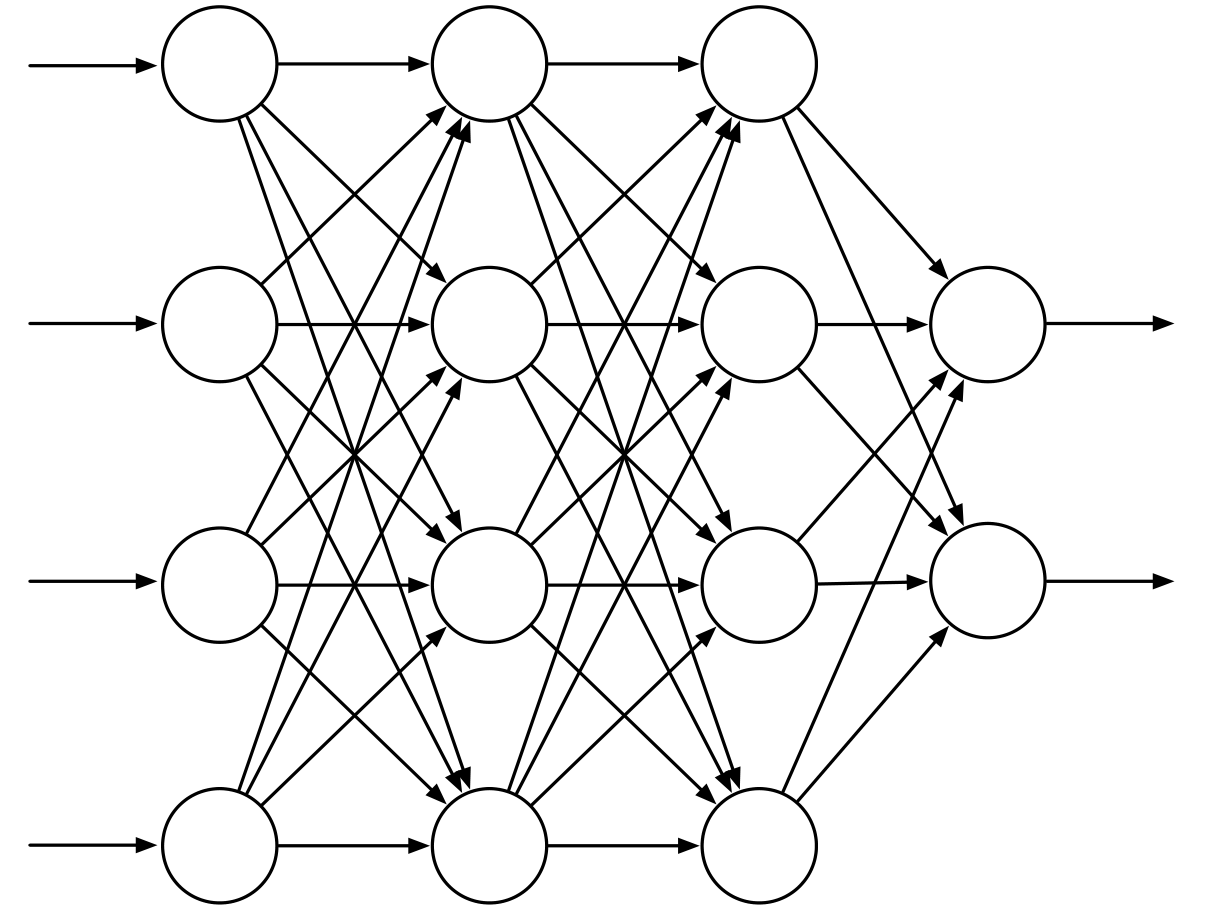
\includegraphics[width=0.7\linewidth]{fig/ann.png}
\caption[Artificial Neural Network]{A sample ANN consisting of four input nodes, two fully connected hidden layers and two output nodes. When approximating the action-value function \(\qpi(s,a)\) the number of input nodes equals the size of the state space and the number of output nodes the size of the action space. The learned connection weights \(\w\) on the arrows between the layers are ommitted in this figure. \protect\footnotemark \label{fig-ann}}
\end{figure}
\footnotetext{Adapted from \textbf{Figure 9.14} from "Reinforcement Learning: An Introduction" by Richard S. Sutton and Andew G. Barto is licencsed under CC BY-NC-ND 2.0 (https://creativecommons.org/licenses/by-nc-nd/2.0/)}
\subsubsection{Further Topics}
\label{sec:org5c7f3ee}
The previous chapters provided a detailed overview of the most important
concepts and mathematical foundations in RL. In the research there are many more
topics that were not covered here. \emph{Eligibility traces} offer a way to more
general learning and faster convergence rates. Almost any TD method can be
extended to use eligibility traces, a popular methods is called Watkins's Q(\(\lambda\))
\cite{watkins89_learn_from_delay_rewar}. \emph{Fitted-Q Iteration} \cite{ernst03_iterat}
combined Q-learning and fitted value iteration with batch-mode RL. In
batch-mode the whole dataset is available offline, contrary to online RL where
the data is acquired by the agent's action in its the environment.
\emph{Actor-critic} methods \cite{sutton84_tempor_credit_assig_reinf_learn} directly
learn a parameterized policy instead of action-values, which inherently allow
continuous state spaces and learning appropriate levels of exploration.
Simultaneously to learning the policy, they approximate a state-value function,
which serves as a "critic" to the learned policy, the "actor". In the current
theory most RL models are single-agent models. For certain real-world
applications multi-agent RL algorithms are necessary to coordinate interaction
between the agents. When multiple learning agents interact with a non-stationary
environment, convergence and stability are a serious problem. \emph{W-learning}
\cite{humphrys96_action_selec_method_using_reinf_learn} is an multi-agent approach
that aims to solve these difficulties.

\clearpage

\section{Empirical Setting}
\label{sec:orgb8ca31f}
This research is embedded in the German carsharing and electricity markets.
Germany is a suitable testbed, since it has a comparably high share of
renewables in its energy mix and is pushing for an energy turnaround (German:
\emph{Energiewende}) since 2010 \cite{bmu10_energ_concep_envir_sound_reliab_affor}
The high renewable energy content in the energy mix causes electricity prices to
be volatile, which makes Germany an attractive location for the use of
VPPs.

Germany is home to the carsharing providers Car2Go\footnote{\url{https://www.car2go.com}} and DriveNow\footnote{\url{https://www.drive-now.com}},
which operate large EV fleets across the globe. It has been argued that electric
carsharing can simultaneously solve several traditional mobility and
environmental problems and are an important element of future smart cities
\cite{firnkorn15_free_float_elect_carsh_fleet_smart_cities}. Further, it is widely
regarded that the future of mobility will be electric, shared, smart and
eventually autonomous \cite{burns13_sustain_mobil,sterling18_three_revol}.
Carsharing providers are already contributing to the first two points by
operating large fleets of electric vehicles. This research addresses the third
point: Using electric carsharing fleets to smartly participate in electricity
markets. Carsharing providers, like Car2Go and DriveNow, operate their
carsharing fleets in a free-float model, which allows customers to pick up and
drop vehicles at any place within the operating zone of the provider.
\red{Free float carsharing is inherently uncertain, additional challenge.}
Customers pay by the minute and are offered incentives to park the EVs at
charging stations at the end of their trip.


We obtained real-world trip data from Daimler's carsharing service Car2Go.
Additionally, we collected freely available balancing market data from the GCRM
platform website \url{https://regelleistung.net}. The data of the EPEX Spot market
have kindly been provided by ProCom GmbH\footnote{\url{https://procom-energy.de}} for research purposes. In the
next chapters the different datasets are described, as well the most important
processing steps outlined.

\subsection{Electronic Vehicle Fleet Data \label{sec-data-car2go}}
\label{sec:orgfa7d909}
The Car2Go dataset consists of GPS data of around 500 Smart ED3 Fortwo vehicles
in Stuttgart. These subcompact cars are equipped with a 17.6kWh battery and a
standard 3.6kW on-board charger. They fully charge in about six to seven hours
and can reach a maximum driving distance of 145km according to the manufacturer.
When equipped with an additional 22kW fast charger the charging time reduces to
about an hour.

\begin{sidewaystable}[hp]
    \caption{Sample Raw Car2Go Data in Stuttgart \label{table-car2go-raw}}
    \centering
    \begin{tabular}{c|ccccccc}
      \hline
      \hline
      Number Plate & Timestamp & Latitude & Longitude & Street & Zip Code & Charging & SoC (\%)\\
      \hline
      S-GO2471 & 24.12.2017 20:00 & 9.19121 & 48.68895 & Parkplatz Flughafen & 70692 & no & 94\\
      S-GO2471 & \ldots{} & \ldots{} & \ldots{} & \ldots{} & \ldots{} & \ldots{}. & \ldots{}\\
      S-GO2471 & 24.12.2017 20:05 & 9.19121 & 48.68895 & Parkplatz Flughafen & 70692 & no & 94\\
      S-GO2471 & 24.12.2017 20:10 & 9.19121 & 48.68895 & Parkplatz Flughafen & 70692 & no & 94\\
      S-GO2471 & 24.12.2017 23:05 & 9.15922 & 48.78848 & Salzmannweg 3 & 70192 & no & 71\\
      S-GO2471 & 24.12.2017 23:10 & 9.15922 & 48.78848 & Salzmannweg 3 & 70192 & no & 71\\
      S-GO2471 & 25.12.2017 00:40 & 9.17496 & 48.74928 & Felix-Dahn-Str. 45 & 70597 & yes & 62\\
      S-GO2471 & 25.12.2017 00:45 & 9.17496 & 48.74928 & Felix-Dahn-Str. 45 & 70597 & yes & 64\\
      S-GO2471 & \ldots{} & \ldots{} & \ldots{} & \ldots{} & \ldots{} & \ldots{}. & \ldots{}\\
      S-GO2471 & 25.12.2017 06:50 & 9.17496 & 48.74928 & Felix-Dahn-Str. 45 & 70597 & no & 100\\
      S-GO2471 & 25.12.2017 08:25 & 9.2167 & 48.78742 & Friedenaustraße 25 & 70188 & no & 42\\
      \hline
      \hline
    \end{tabular}

    \bigskip\bigskip  % provide some separation between the two tables

    \caption{Sample Processed Car2Go Trip Data in Stuttgart \label{table-car2go-processed}}
    \centering
    \begin{tabular}{cc|ccccc}
      \hline
      \hline
      Number Plate & Trip & Start Time & Start Latitude & Start Longitude & Start SoC (\%)\\
      \hline
      S-GO2471 & 1 & 24.12.2017 20:10 & 9.19121 & 48.6890 & 94\\
      S-GO2471 & 2 & 24.12.2017 23:10 & 9.15922 & 48.7885 & 71\\
      S-GO2471 & 3 & 25.12.2017 06:50 & 9.17496 & 48.7493 & 66\\
      \hline
      Number Plate & Trip & End Time & End Latitude & End Longitude & End SoC (\%)\\
      \hline
      S-GO2471 & 1 & 24.12.2017 23:05 & 9.15922 & 48.7885 & 71\\
      S-GO2471 & 2 & 25.12.2017 00:40 & 9.17496 & 48.7493 & 62\\
      S-GO2471 & 3 & 25.12.2017 08:25 & 9.2167 & 48.7875 & 42\\
      \hline
      Number Plate & Trip & Trip Duration (min) & Trip Distance (km) & Trip Charge (\%) & End Charging\\
      \hline
      S-GO2471 & 1 & 175 & 33.35 & 23 & no\\
      S-GO2471 & 2 & 90 & 13.05 & 9 & yes\\
      S-GO2471 & 3 & 155 & 29 & 20 & no\\
      \hline
      \hline
    \end{tabular}
\end{sidewaystable}

In Table \ref{table-car2go-raw} the raw data is displayed, as we have obtained it
by Car2Go. The dataset contains spatio-temporal attributes, such as timestamp,
coordinates, and the address of the EVs in 5 minute intervals. Additionally,
status attributes of the interior and exterior are given (not displayed).
Especially relevant for our research is the state of charge (\(SoC\), in \%) and
information whether the EV is plugged into a charging station. Note that the
data only contain EVs that are \emph{available for rent}, i.e., they are not
currently rented out by a customer. EVs which are parked at a charging station
are also not available until they have charged up to approximately 70\% SoC. For
further analysis, individual trips had to be reconstructed using the GPS data of
the cars, moreover we inferred trip distances and trips prices based on Car2Go
specifications. See Appendix \ref{app-data-processing} for a detailed listing of
the executed preprocessing steps.


\subsection{Balancing Market Data \label{sec-data-balancing}}
\label{sec:org91f9504}
In this research, we use market balancing data from the German secondary reserve
market. The following chapter will give an overview of the dataset and
preprocessing steps that were taken. The data encompasses weekly lists of
anonymized bids between 01.06.2016 and 01.01.2018 and a dataset of activated
control reserve in Germany during the same period. For a detailed description
about the market design of balancing markets refer to Chapter
\ref{sec-balancing-market}.

The bidding data consists of the traded electricity product, the offered
capacity \(\Pb{}\) (MW), the capacity price \(\cp{}\) (\(\emw\)), and the
energy price \(\ep{}\) (\(\emwh\)) of each bid. Four different products
are traded, which are a combination of positive control reserve (feed
electricity into the grid) or negative control reserve (take electricity from
the grid) and the provided time segment (peak or non-peak hours). Since negative
prices are allowed on the secondary operating reserve market, the payment
direction is included as well. Moreover, information about the amount of
capacity that was accepted, i.e., either partially or fully, is listed. Bids,
which were not accepted by the TSOs are not listed. An exemplary excerpt of the
dataset is displayed in Table \ref{table-operating-reserve}.

\begin{longtable}{c|ccccc}
\caption[Secondary Operating Reserve Market Data]{List of Bids of the German Secondary Reserve Market for the tender period 04.12.2017 - 11.12.2017. \label{table-operating-reserve}}
\\
\hline
\hline
Product & Capacity Price & Energy Price & Payment & Offered & Accepted\\
\hline
\endfirsthead
\multicolumn{6}{l}{Continued from previous page} \\
\hline

Product & Capacity Price & Energy Price & Payment & Offered & Accepted \\

\hline
\endhead
\hline\multicolumn{6}{r}{Continued on next page} \\
\endfoot
\endlastfoot
\hline
NEG-HT & 0 & 1.1 & TSO to bidder & 5 & 5\\
NEG-HT & 10.73 & 251 & TSO to bidder & 15 & 15\\
NEG-HT & 200.3 & 564 & TSO to bidder & 22 & 22\\
\ldots{} & \ldots{} & \ldots{} & \ldots{} & \ldots{} & \ldots{}\\
NEG-NT & 0 & 21.9 & Bidder to TSO & 5 & 5\\
NEG-NT & 0 & 22.4 & Bidder to TSO & 5 & 5\\
\ldots{} & \ldots{} & \ldots{} & \ldots{} & \ldots{} & \ldots{}\\
POS-NT & 696.6 & 1200 & TSO to bidder & 5 & 5\\
POS-NT & 717.12 & 1210 & TSO to bidder & 10 & 7\\
\hline
\hline
\end{longtable}

In this study, we assume that bidding on 15-minute intervals in secondary
operating reserve auctions will be possible in future energy markets. As
mentioned in Chapter \ref{sec-balancing-market}, the market design of the GCRM
secondary operating reserve tender was adjusted in 2017. Daily tenders with
4-hour bidding intervals were introduced in favor of weekly tenders with only
two time segments. This change represents the trend by the TSOs to change the
market design in order to better include RES into the operating reserve markets
\cite{agricola14_dena_ancil_servic_study}. Due to the volatility of renewable
electricity generation, providers are naturally dependent on accurate short-term
forecasts, which are only possible with short tender periods and fine-grained
bidding intervals.

In order to estimate the upper bound of profits that the EV fleet can earn by
participating in the secondary operating reserve market, the \emph{critical prices}
\(\ccp{}\) and \(\cep{}\) were determined for each auctioned interval. Following
\textcite{brandt17_evaluat_busin_model_vehic_grid_integ}, we define \(\ccp{}\)
(\(\emw\)) as the capacity price of the bid that was just barely
accepted, whereas \(\cep{}\) (\(\emwh\)) is the highest energy price
that was payed for activated control reserve during that interval. For every
15-minute interval within the given tender period of one week, the activated
control reserve in that interval was matched with the accepted bids in that
tender period. At the point where supply, i.e., offered capacity of bids, met
demand, i.e., activated control reserve, the critical price \(\cep{}\) was
determined.

\emph{Example}: The assumed critical prices for the secondary operating reserve
tender interval of the 6\textsuperscript{th} December 2017 between 08:00 and 08:15 are obtained
as follows: Three suppliers submitted a reserve capacity of 5MW, 15MW and 22MW
respectively (see Table \ref{table-operating-reserve}). The critical capacity
price \(\ccp{}\!=\!200.3\emw\) is determined by the capacity price of the last
(third) accepted bid in that time segment. The TSO reported that 18MW of control
reserve were activated between 08:00 and 08:15. Hence, the second bid determines
the critical energy price \(\cep{}\!=\!251\emwh\), as control reserve capacity
gets activated according to ascending order of the submitted energy prices. In
this example the second bidder would get compensated with:
\(R\!=\!R^c + R^e\!=\!(10.73\emw\!\times\!15\mw) +
(251\emwh\!\times13\mw\!\times\!0.25\text{h})\!=\! 976.7\eur\). Note that
the second bidder get compensated for providing 13MW for 15 minutes (0.25h),
instead of the submitted 15MW, since in total only 18MW of control capacity was
activated, which was partly fulfilled by the 5MW of the first bidder.

\subsection{Spot Market Data \label{sec-data-intraday}}
\label{sec:orgd57dfa1}
The data from the EPEX Spot Intraday Continuous encompass order books and
executed trades from 01.06.2016 until 01.01.2018. An extract of the data can be
found in Appendix \ref{app-data-tables}. The list of trades contains information
on the unit price \(\up{}\) (\(\emwh\)), the quantity (kW) and the traded product
(hourly, quarterly or block). In this research, we focus on quarterly product
times (15-minute intervals), as they provide the highest flexibility. Fleet
controllers can promptly react to fluctuant electricity demand of the EV fleet
by accurately adjusting the bid quantities. Future research could also consider
other electricity products if lower prices justify decreased flexibility at that
point in time. Additionally, the TSOs of the buyer and seller are listed in the
dataset. They are only relevant if special conditions between TSO apply, for
example when delivering electricity to other countries.

\begin{figure}[hp]
\centering
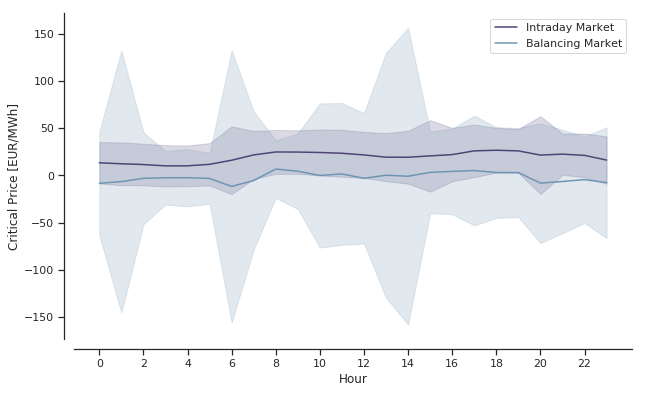
\includegraphics[width=1\linewidth]{fig/critical-prices.png}
\caption[Critical electricity prices]{Daily critical electricity market prices (average, standard deviation) from June 6, 2016 to January 1, 2018. Highly volatile prices, e.g., between 12:00 and 14:00, illustrate the benefits of an integrated trading strategy, which considers trading on both markets depending on the market conditions.}
\end{figure}

On the spot market, electricity trades can have a very short lead time of up to
5 minutes before delivery. This market characteristic is beneficial for our
proposed trading strategy, since it allows the EV to procure electricity in
almost real time. The controller can submit bids to the market, with accurate
estimations of available charging capacity up to five minutes ahead. Similarly
to the balancing market, the critical price \(\cup{}\) has to be determined for
all intraday trading intervals. The critical unit price \(\cup{}\) is defined as
the lowest price of all executed trades.
\begin{equation*}
    \cup{} \defeq \min_{t \in \cal{T}} \up{t} \text{ ,}
\end{equation*}
where \(\cal{T}\) is the set of all trades in a bidding interval. \emph{Example:} The
critical unit price of the trades listed in Appendix \ref{app-data-tables} is
\(\cup{} \!=\!51.00 \emwh\) (trades 8031392, 8031387 and 8031375). All buyers that
submitted bids with a price higher than the critical unit price, successfully
procured electricity. Hence, accurate forecasts of the critical price allow to
optimize the bidding behavior. For a detailed description of the intraday
continuous market see Chapter \ref{sec-spot-market}.

\clearpage

\section{Model}
\label{sec:org552bd44}
The following chapter will introduce the model of this research. In its essence,
we propose a solution for EV fleet providers to utilize a VPP portfolio to
profitably provide balancing services to the grid on multiple markets. A control
mechanism procures energy from electricity markets, allocates available EVs to
VPPs, and intelligently dispatches EVs to charge the acquired amount of energy.
The model employs a RL agent that learns an optimal bidding strategy by
interacting with the electricity markets and reacts to changing rental demand of
the EV fleet. This chapter is structured as follows: The information assumptions
are listed first, the control mechanism is explained next, and finally, the RL
approach is described in detail. The used notation in this chapter can be found
in Table \ref{table-notation}.

We formulate the problem as a \emph{controlled EV charging} problem. The EV fleet
operator represents the \emph{controller}, which aims to charge the fleet at minimal
costs. First, the controller predicts the amount of energy it can charge in a
given \emph{market period} \(h\). The length of the market period \(\Delta h\) and the
market closing time depend on the considered electricity market. Second, the
controller places bids on one or multiple markets to procure the predicted
amount of energy. Lastly, at electricity delivery time, the controller
communicates with the EV fleet to control the charging in real-time. Online EV
\emph{control periods} \(t\) are typically shorter than market periods. In the
empirical case that we consider, the market periods are 15 minutes long, while
the EV control periods last 5 minutes. Nonetheless, the presented approach
generalizes to other period lengths. During each control period, the controller
has to take decisions which individual EVs it should dispatch to charge the
procured amount of electricity. In times of unforeseen rental demand, this
decision implies trading off commitments to the markets with compromising
customer mobility by refusing customer rentals.


\begin{longtable}{p{0.11\linewidth}|p{0.75\linewidth}|c}
\caption[Table of Notation]{Table of Notation \label{table-notation}}
\\
\hline
\hline
Symbol & Description & Unit\\
\hline
\endfirsthead
\multicolumn{3}{l}{Continued from previous page} \\
\hline

Symbol & Description & Unit \\

\hline
\endhead
\hline\multicolumn{3}{r}{Continued on next page} \\
\endfoot
\endlastfoot
\hline
\(t\) & Control period. & -\\
\(h\) & Market period. & -\\
\(T\) & Number of control periods in a market period. & -\\
\(H\) & Number of market periods in day. & -\\
\(N_h\) & Total number of market periods. & -\\
\(\Delta t\) & Length of control period. & hours\\
\(\Delta h\) & Length of market period. & hours\\
\hline
\(\Pb{h}\) & Amount of balancing power offered on the balancing market. & kW\\
\(\ccp{h}\) & Critical capacity price in market period \(h\). & \(\emw\)\\
\(\cep{h}\) & Critical energy price in market period \(h\). & \(\emwh\)\\
\(\Pi{h}\) & Amount of power offered for the unit on the intraday market. & kW\\
\(\cup{h}\) & Critical unit price in market period \(h\). & \(\emwh\)\\
\(\Eb{h}\) & Amount of energy charged from balancing market in market period h. & MWh\\
\(\Ei{h}\) & Amount of energy charged from the intraday market in market period h. & MWh\\
\hline
\(\fP{t}\) & Amount of available fleet charging power in control period \(t\). & kW\\
\(\fPhat{t}\) & Predicted amount of available fleet charging power in control period \(t\). & kW\\
\hline
\(\Cb{h}(P)\) & Cost function for procuring electricity from the balancing market. & \(\eur\)\\
\(\Ci{h}(P)\) & Cost function for procuring electricity from the intraday market. & \(\eur\)\\
\(\oc\) & Opportunity costs of lost rental of EV \(i\) in control period \(t\). & \(\eur\)\\
\(\beta_h\) & Imbalance costs in market period \(h\). & \(\eur\)\\
\hline
\(\lb{h}\) & Balancing market risk factor. & \([0,1]\)\\
\(\li{h}\) & Intraday market risk factor. & \([0,1]\)\\
\(\theta_{\lambda}\) & Set of risk factors for all market periods \(h\!\in\!\{1,...,N_h\}\). & -\\
\(\Cf{}(\theta_{\lambda})\) & Cost function for the fleets total costs over all market periods \(h\). & \(\eur\)\\
\(\Cf{h}\) & Total accumulated fleet costs until market period \(h\). & \(\eur\)\\
\hline
\(i\) & Electric Vehicle. & -\\
\(\F\) & Set of all EVs in the fleet & -\\
\(\c\) & Dummy variable if EV is connected to a charging station. & 0/1\\
\(\omega_{i}\) & Amount of electricity stored in EV. & \(\kwh\)\\
\(\Omega\) & Maximum battery capacity of EV. & \(\kwh\)\\
\(\delta\) & Charging power of EV at the charging station. & \(\kw\)\\
\(p^{ind}\) & Industry tariff & \(\ekwh\)\\
\hline
\end{longtable}

\subsection{Assumptions \label{sec-model-assumptions}}
\label{sec:orgba89ace}

In order to evaluate and operationalize our model, the following assumptions
about the available information and the electricity market mechanism are taken:
\subsubsection{Information Assumptions}
\label{sec:orgb99e6e2}

\begin{enumerate}
\item Mobility demand

The controller is able to forecast the mobility demand of the EV fleet with
different time-horizons based on historical data. More specifically, it can
predict the amount of plugged-in EVs and consequently the available charging
power \(P^{fleet}_t\) of the fleet at control period \(t\). The prediction
accuracy is increasing with shorter time horizons, from uncertain predictions
one week ahead to very accurate predictions 30 minutes ahead. Past research
presented successful mobility demand forecast algorithms in the context of
free-float carsharing
\cite{kahlen18_elect_vehic_virtual_power_plant_dilem,kahlen17_fleet,wagner16_in_free_float}.
\item Critical electricity prices

The controller is able to forecast electricity prices of spot and balancing
markets based on historical data. More specifically, it can estimate the
critical prices \(\ccp{h}\), \(\cep{h}\), and \(\cup{h}\) for each market period
with perfect accuracy (see Chapter \ref{sec-data-balancing} and Chapter
\ref{sec-data-intraday} for the critical price definitions). Electricity price
forecasting is an extensively studied research area with well-advanced
prediction algorithms
\cite{weron14_elect_price_forec,avci18_manag_elect_price_model_risk}.
\end{enumerate}
We are confident that taking the above assumptions is viable, assuming available
forecasting information is common practice in the VPP and EV fleet charging
literature, for example
\textcite{vandael15_reinf_learn_heuris_ev_fleet,mashhour11_biddin_strat_virtual_power_plant_1,tomic07_using_fleet_elect_drive_vehic_grid_suppor,pandzic13_offer_model_virtual_power_plant}.

\subsubsection{Market Assumptions}
\label{sec:org316d728}
\begin{enumerate}
\item Balancing market

The controller is able to submit bids of any quantity for single 15-minute
market periods 7 days ahead. Since the critical capacity and energy prices
are available (previous paragraph), the controller submits bids in the form
\(bid\!=\!(\Pb{},\ccp{},\cep{})\). Submitting a bid with the critical capacity
price ensures that the bid will always get accepted by the TSOs. Submitting
the bid with the critical energy price ensures that the balancing power will
always get fully activated, which allows the fleet to charge at the submitted
price for the market periods length.

\item Intraday market

The controller submits bids to the intraday market 30 minutes ahead. The bids
are submitted in the form \(bid\!=\!(\Pi{},\cup{})\). We assume that the order
to buy will always get matched until the minimal lead time of the trade
(e.g., 5 minutes on the EPEX Spot Intraday Continuous). In reality, this is
not always the case since trades are executed immediately and it is not
guaranteed that a matching order to sell is submitted between the bidding
time and the minimal lead time.
\end{enumerate}
In essence, we are assuming that the controller always submits the optimal bid
at the right time. In other words, every bid leads to the successful procurement
of the desired amount of electricity. This assumption provides an upper bound
for the fleet profits from trading EV battery storage on the electricity
markets. However, the upper bound is only influenced by the accuracy of the
electricity price forecasting algorithm, a research area that well exceeds the
scope of this work. Furthermore, we assume that the controller is a price-taker.
Due to the limited size of its bids, it is lacking the market share to influence
prices on the markets. Similar assumptions have been made by
\textcite{brandt17_evaluat_busin_model_vehic_grid_integ} and
\textcite{vandael15_reinf_learn_heuris_ev_fleet}.
\subsection{Control Mechanism \label{sec-model-mechanism}}
\label{sec:orga143de1}
The control mechanism constitutes the core of this research. It can be seen as a
decision support system that can be deployed at an EV fleet operator to centrally
control the charging of its fleet. Figure \ref{fig-control-mechanism} depicts the
control mechanism, which is divided into three distinct phases:

The first phase, \emph{Bidding Phase I}, takes place just before the closing time of
the balancing market, once every week (e.g., Wednesdays at 3pm at the GCRM). In
this phase, the controller can place bids for every market period \(h\) of the
following week on the balancing market. The second phase, \emph{Bidding Phase II},
takes places in every market period of \(\Delta{h}\!=\!15\) minutes. At this
point, the controller has the opportunity to place bids to the intraday market
for the market period 30 minutes ahead. The third phase, \emph{Dispatch Phase}, takes
places in every control period of \(\Delta{t}\!=\!5\) minutes. In this phase the
controller has to dispatch available EVs to charge the procured electricity from
the markets. The phase involves allocating individual EVs to the VPP and
potentially refusing customer rentals to assure that all market commitments can
be fulfilled.

The following chapters will highlight the important parts of the three phases
and provide detailed explanation and mathematical formulations.

\begin{figure}[p]
\centering
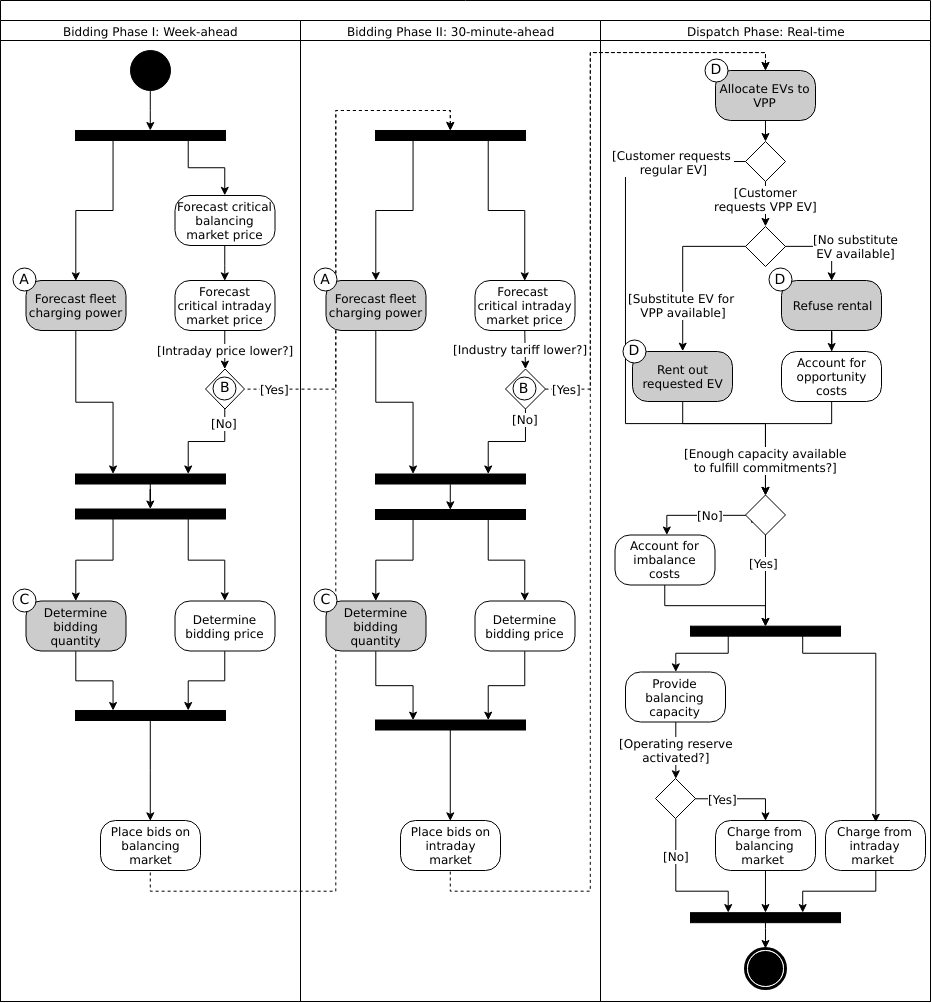
\includegraphics[width=1.05\linewidth]{fig/control-mechanism.png}
\caption[Control Mechanism]{Control Mechanism \label{fig-control-mechanism}}
\end{figure}

\subsubsection{Fleet Charging Power Prediction}
\label{sec:org90d15ca}

In a first step, the controller has to predict the available fleet charging
power for the market period of interest (see\circled{A} in Figure
\ref{fig-control-mechanism}). The actual available fleet charging power \(\fP{t}\)
in a control period \(t\) is given by the number of EVs that are connected to a
charging station, with enough free battery capacity to charge the next control
period \(t\!+\!1\).

When the controller procures electricity from the markets, the fleet has to
charge with the committed charging power during all control periods of the
market period \(h\), otherwise imbalance costs occur. To minimize the risk of not
being able to charge the committed amount of energy during the whole market
period, the predicted fleet charging power in a market period is defined as the
minimal predicted fleet charging power of all control periods in that market
period:
\begin{equation}
    \fPhat{h} \defeq \min_{n \in \{1, .., T\}} \fPhat{t + n} \text{ ,}
\end{equation}
where \(h\) is the market period of interest, \(t\) its first control period and \(T\)
the number of control periods in a market period.



\subsubsection{Market Decision}
\label{sec:orgb77d27e}
In a second step, the controller has to decide from which market it should
procure the desired amount of energy (see\circled{B} in Figure
\ref{fig-control-mechanism}). Therefore, it compares the costs for charging
electricity from the balancing market with the costs for charging from the
intraday market. The cost function for procuring electricity from the balancing
market is defined as follows:
\begin{equation} \label{eq-cost-balancing}
\begin{split}
    \Cb{h}(P) &\defeq -(P\!\times\!10^{-3} \times \ccp{h}) + (\Eb{h} \times \cep{h}) \\
    &= -(P\!\times\!10^{-3} \times \ccp{h}) + (P \frac{\Delta h}{10^{3}} \times \cep{h}) \text{ ,}
\end{split}
\end{equation}
where \(P\) (kW) is the amount of offered balancing power. The first term of the
equation corresponds to the compensation the controller retrieves for keeping
the balancing capacity available, while the second term corresponds to the costs
for charging the activated balancing energy \(\Eb{h}\) (MWh). Energy is power over
time, hence \(\Eb{h}\) can be substituted with \(P\) times the market periods length
\(\Delta{h}\), divided by the unit conversion term from kW to MW. Note that the
critical energy price \(\cep{}\!\in\!\Re\), can also take negative values,
resulting in profits for the fleet, while the critical capacity price
\(\ccp{}\!\in\! \Re^+_0\) is never negative and therefore never results in
costs for the fleet.

The cost function for charging from the intraday market is defined similarly to
\eqref{eq-cost-balancing}:
\begin{equation}
\begin{split}
    \Ci{h}(P) &\defeq \Ei{h} \times \cup{h} \\
    &= P \frac{\Delta h}{10^{3}}\times \cup{h}
\end{split}
\end{equation}
Again, depending on the market situation, \(\cup{}\!\in\!\Re\) can either be
negative or positive, resulting in costs or profits for the fleet. Contrarily to
the balancing market, on the intraday market the fleet does not get compensated
for keeping the charging power available; only the charged energy affects the
costs. If the costs for charging from the balancing market 7 days ahead
\(\Cb{h+(7\!\times\!H)}(\fPhat{h+(7\!\times\!H)})\) are higher than the costs of
charging from the intraday market at the same market period \(\Ci{h +
(7\!\times\!H)}(\fPhat{h+(7\!\times\!H)})\), the controller does not procure
electricity from the balancing market.

\subsubsection{Determining the Bidding Quantity}
\label{sec:orgbe52a85}
In a third step, the controller has to take a decision on the amount of energy
it should procure from the markets (see\circled{C} in Figure
\ref{fig-control-mechanism}). Determining the bidding quantity is the core
challenge of the controlled charging problem. The bidding quantity determines
the profits that can be made by charging at a cheaper market price than the
flat industry tariff. On one hand, the controller aims to maximize its profits
by procuring as much electricity as possible from the markets. On the other
hand, it needs to balance the risk of (a) procuring more energy that it can
maximally charge and (b) not procuring enough energy from the market to
sufficiently charge the fleet.

In case (a), the fleet is facing costs of compromising customer mobility, or
worse, high imbalance penalties from the markets. Renting out EVs is
considerably more profitable than using their batteries as a VPP. Refusing
customer rentals, in order to fulfill market commitments, induces opportunity
costs of lost rentals \(\rho\) on the fleet. Imbalance costs \(\beta\) occur, when
the fleet can not charge the committed amount energy at all, even with refusing
rentals. In case (b), the fleet also faces opportunity costs of lost rentals
when individual EVs do not have enough SoC for planned trips of arriving
customers.

The controller faces additional risks by bidding one week ahead on the balancing
market, in contrast to only 30 minutes ahead on the intraday market: Predictions
of available charging power are more uncertain with the larger time horizon. To
account for all mentioned risks, we introduce a \emph{risk factor} \(\lambda \in
\Re_{0 \leq \lambda \leq 1}\), where \(\lambda\!=\!0\) indicates no risk, and
\(\lambda\!=\!1\) indicates a high risk. The controller determines the bidding
quantity \(\Pb{h}\) by discounting the predicted available fleet charging power
\(\fPhat{h}\) with the possible risk \(\lambda_{h}\) of imbalance or opportunity
costs:
\begin{equation} \label{eq-model-pb}
  \Pb{h} \defeq
  \begin{cases}
    0, & \text{if}\ \Cb{h}(\fPhat{h}) \geq \Eb{h}10^3 \times p^{ind}\\
    0, & \text{if}\ \Cb{h}(\fPhat{h}) \geq \Ci{h}(\fPhat{h})\\
    \fPhat{h} \times (1\!-\!\lb{h}), & \text{otherwise}
  \end{cases}
\end{equation}
where \(h\) is the market period of interest one week ahead. If the controller can
buy electricity at the intraday market at a lower price, it does not place a bid
at the balancing market. If the controller can charge cheaper at the regular
industry tariff \(p^{ind}\), it does not place a bid either. In all other cases, the
controller submits \(\Pb{h}\) to the market.

The bidding quantity for the intraday market \(\Pi{h}\) depends on the previously
committed charging power \(\Pb{h}\) and the newly predicted charging power
\(\fPhat{h}\):
\begin{equation} \label{eq-model-pi}
  \Pi{h} \defeq
  \begin{cases}
    0, & \text{if}\ \Ci{h}(\fPhat{h}\!-\!\Pb{h}) \geq \Ei{h}10^3 \times p^{ind}\\
    (\fPhat{h}\!-\!\Pb{h}) \times (1\!-\!\li{h}), & \text{otherwise}
  \end{cases}
\end{equation}
where \(h\) is the market period of interest 30 minutes ahead. Note that any
amount of electricity that the controller procured from the balancing market
\(\Pb{h}\), does not need to be bought from intraday market for the same market
period. Since the predicted charging power \(\fPhat{h}\) is expected to be more
accurate 30 minutes ahead than one week ahead, the controller is able to correct
bidding errors it made in the first decision phase, and optimally charge the
whole EV fleet.

\subsubsection{Dispatching Electronic Vehicle Charging}
\label{sec:orgcea3d70}
In the last step, at electricity delivery time, the EVs have to be assigned to
the VPP and be \emph{dispatched} to charge (see\circled{D} in Figure
\ref{fig-control-mechanism}). Therefore the controller needs to detect how many
EVs are eligible to be used as VPP in the control period \(t\). An EV \(i\) is
eligible if (a) it is connected to a charging station (\(\c\) = 1), and (b) it has
enough free battery storage available (\(\Omega\!-\!\omega_{i}\)) to charge the
next control period. Hence, the VPP is defined as:
\begin{equation}
    V\!P\!P \defeq \{i\in\F \;|\; \c = 1 \vee \Omega\!-\!\omega_{i}\!\geq\!\gamma\Delta{t}\} \text{ ,}
\end{equation}
where \(\gamma\Delta{t}\) (kWh) denotes the amount of energy that can be charged
with the charging speed of \(\gamma\) (kW) in control period \(t\). \(\gamma\) is
limited by either the EVs build-in charger, or the charging power of the
connected charging station. In this model we assume \(\gamma\) is equal for all
considered EVs and charging stations. \emph{Example:} Assuming a charging power of
\(\gamma\!=\!3.3\kw\), an EV battery capacity of \(\Omega\!=\!17.6\kwh\), and
control periods of 5 minutes, the amount of energy charged in one control period
is \(3.3\kw\!\times\frac{5}{60}\text{h}\!=\!0.275\kwh\). Hence, the maximal
battery capacity to be eligible for VPP use is \(17.6-\!0.275\!=\!17.325\kwh\).

Remember that the fleet has to provide the total committed charging power
\(\Pb{h}\!+\!\Pi{h}\) across all control periods \(t\) of the market period \(h\),
independent of which individual EVs are actually charging the electricity. This
fact allows the controller to dynamically dispatch EVs every control period and
react to unforeseen rental demand. If a customer wants to rent out an EV that is
assigned to the VPP, the controller only has to refuse the rental, if no other
EV is available to charge instead. When no replacement EV is available, the
controller has to account for lost rental profits \(\oc\). If the VPPs total
amount of available charging power \(\vpp{t}\!\times\!\gamma\) is not sufficient to
provide the total market commitments \(\Pb{h}\!+\!\Pi{h}\), the fleet gets charged
imbalance costs \(\beta_{h}\). Otherwise all the committed energy can be charged
by the VPP.

\subsubsection{Evaluating the Bidding Risk}
\label{sec:orgcbb1f68}
The controllers main goal is to choose the risk factors \(\lb{h}\), \(\li{h}\)
for every market period \(h\), that minimize the cost of charging, while avoiding
the risks of lost rental profits \(\oc\) or imbalance costs \(\beta_h\). The total
fleet costs are defined as follows:
\begin{equation} \label{eq-model-fleetcosts}
    \Cf{}(\theta_{\lambda}) \defeq \sum^{N_h}_h
    \bigg[ \Cb{h}(\Pb{h}) + \Ci{h}(\Pi{h}) + \beta_{h}
    + \sum_t^{T} \sum_i^{|\F|} \oc \bigg] \text{ ,}
\end{equation}
where \(\theta_{\lambda}\!\in\!\Re_{0 \leq \lambda \leq 1}^{2 \times N_h}\) is the
matrix of the risk factors \(\lb{h}\), \(\li{h}\) for all considered market periods
\(N_h\). \(\F\) denotes the set of all EVs \(i\) in the fleet and \(|\F|\) the fleet
size. The costs for charging \(\Cb{h}(\Pb{h})\), \(\Ci{h}(\Pi{h})\) are clearly
dependent on the chosen risk factors \(\lb{h}\), \(\li{h}\) (see
\eqref{eq-model-pb} and \eqref{eq-model-pi}). In summary, the problem can be
formulated as minimizing the total costs of the fleet, by choosing the optimal
set of risk factors \(\theta_{\lambda}\):
\begin{equation}
\begin{aligned}
    & \underset{\theta_{\lambda}}{\text{minimize}}
    && \Cf{}(\theta_{\lambda}) \\
    & \text{subject to}
    && 0 \leq \lb{h} \leq 1, \; \forall \lb{h} \in \theta_{\lambda}\\
    &&& 0 \leq \li{h} \leq 1, \; \forall \li{h} \in \theta_{\lambda}\\
\end{aligned}
\end{equation}
Solving this optimization problem with common methods like stochastic
programming is a difficult task, assuming that complete information of available
charging power and future electricity market prices is not always available.
Since one goal of this research is to develop a model that can be applied to
previously unknown settings and learn from uncertain environments, as mobility
and electricity markets, we chose to solve the problem with a RL approach that
is explained in detail in Chapter \ref{sec-model-rl}.

\subsubsection{Example}
\label{sec:orgb88ff54}
At 3pm on the 9\textsuperscript{th} of August 2017, the controller enters the first bidding
phase for the market period \(h\) = \emph{16.08.2017 15:00-15:15}. It predicts that at
that point in time 250 EVs are connected to a charging station, resulting in
900kW available fleet charging power (\(\fPhat{h}\!=\!900\kw\)), given the
charging power of 3.6kW per EV. Assuming the available critical prices are
\(\ccp{h}\!=\!5\emw\), \(\cep{h}\!=\!-10\emwh\), and \(\cup{h}\!=\!10\emwh\) in that
market period, the controller now evaluates the cheapest charging option. The
flat industry electricity tariff is assumed to be \(p^{ind}\!=\!0.15\ekwh\). The
costs for charging with the maximal predicted amount of available power
\(\fPhat{h}\) from the balancing market (\(\Cb{h}(900\kw)\!=\!-6.25\eur\)) are less
than charging from the intraday market (\(\Ci{h}(900\kw)\!=\!2.25\eur\)) or
charging at the industry tariff
(\(900\kw\!\times\!0.25\text{h}\!\times\!0.15\ekwh\!=\!33.75\eur\)). In this
example, the fleet operator will even get compensated for charging its fleet, by
choosing the balancing market.

In the next step, the controller has to submit bids to the balancing market. The
RL agent determined that the risk of bidding on the balancing market is
\(\lb{h}\!=\!0.3\). Consequently, the controller sets the bidding quantity to
\(\Pb{h}\!=\!\fPhat{h}\!\times\!(1\!-\!\lb{h})\!=\!900\kw\!\times0.7\!=\!630\kw\)
and submits a bid to the market and updates its account with
\(\Cb{h}(630\kw)\!=\!-4.725\eur\).

One week later, 30 minutes before electricity delivery time, the controller
enters the second bidding phase. Due to the short time horizon, it predicts with
high accuracy that only \(\fPhat{h}\!=\!810\kw\) is available for the same market
period \emph{16.08.2017-15:00}. By trading at the intraday market, the controller can
now charge the remaining available EVs with a low risk of procuring more energy
than it can maximally charge. At this point in time, the RL agent determines a
remaining risk of \(\li{h}\!=\!0.05\), and sets the bidding quantity to
\(\Pi{h}\!=\!(810\kw\!-\!630\kw)\!\times\!(1\!-\!0.05)\!=\!171\kw\). The
controller procures 171kW from the intraday market and updates its account with
\(\Ci{h}(171\kw)\!=\!0.4275\eur\).

At electricity delivery time, the 16\textsuperscript{th} of August 2017 at 3:00pm, the
controller detects 255 available EVs; EVs which are connected to a charging
station and have enough battery capacity left to be charged in the next control
period. It assigns 223 EVs to provide the total committed 801kW charging power
for the market period time \(\Delta h\) of 15 minutes. During that time, three
customers want to rent out EVs that are allocated to the VPP. The first two
rentals are accepted because two other EVs are available to charge instead. The
third rental has be to refused, since no EV is remaining as substitution. The
controller has to account for the opportunity costs of the lost rental \(\oc\).


\subsection{Reinforcement Learning Approach \label{sec-model-rl}}
\label{sec:org72f4dab}
In the following chapter the developed RL approach is outlined. First, we define
the charging problem as a MDP, and second, the learning algorithm is explained.
Remember that the goal of the controlled charging problem is to choose a set of
risk factors \(\theta_{\lambda}\) that minimize the fleets total costs across all
market periods. The controller is able to influence the costs, by setting the
risk factors \(\lb{}\), \(\li{}\) each market period \(h\). The risk factors influence
the bidding quantities \(\Pb{h}\), \(\Pi{h}\) that the controller submits to the
balancing and intraday market, which in the end determine the fleet costs. The
RL agent decides on the risk factors (i.e., takes an action) based on the
observed state \(\S\) every time step \(h\) (usually denoted as \(t\) in the RL
literature). The optimal set of risk factors is learned by the RL agent through
estimating a policy \(\pi(a|s)\) that maps every state \(s\in\S\) to an action
\(a\in\A\).
\subsubsection{Markov Decision Process Definition}
\label{sec:org59360b1}

MDPs are defined by the state space \(\S\), the action space \(\A\), a set of reward
signals \(\R\) and the state-transition probabilities \(p(s'|a,s)\). When
\(p(s'|a,s)\) is unknown, as it is in our case, it is possible to use a
model-free approach (see Chapter \ref{sec-td-learning}). The state space
compromises the observed information the agent uses to decide on the action it
is going to take. We observed the following factors that are associated with the
bidding risk:
\begin{enumerate}
\item The bidding period's time of the day

In times of volatile customer rental demand (e.g., during rush hour), the
uncertainty on the guaranteed amount of available EVs increases. Bidding for
these periods involves a higher risk of not being able to fulfill market
commitments.
\item The current and estimated future size of the VPP

Large VPPs benefit from the \emph{risk-pooling} effect \cite{kahlen17_fleet}.
Intuitively that means, larger VPPs are exposed to smaller risks: They have
an increased probability that "lost" charging power, due to unforeseen
rentals, can be substituted by the EVs of the VPP.
\end{enumerate}

Since forecasts of available charging power are already available, we define the
predicted VPP size \(\vpphat{h}\) as the as the necessary amount of EVs to provide
the predicted charging power \(\fPhat{}\) in time period \(h\):
\begin{equation}
    \vpphat{h} \defeq \left\lceil\frac{\fPhat{h}}{\gamma}\right\rceil \text{ ,}
\end{equation}
where \(\gamma\) is the charging power per EV. \emph{Example:} When the controller
predicted 910kW available charging power, the estimated future
size of the VPP to charge with the predicted power is  \texttt{ceil(} \(\!910\kw /
3.6\kw\!\) \texttt{)} = 253.


The state space is then defined as
the set of all valid values of the elements of the following tuple:
\begin{equation}
    \S \defeq \left\langle t(h), \vpp{h}, \vpphat{h+2}, \vpphat{h+(7\!\times\!H)}\right\rangle \text{ ,}
\end{equation}
where:
\begin{itemize}
\item \(t(h)\) is the current daytime in hours, with discrete values in the range
\(\big[0,\;23\big] \in \Ne\).
\item \(|VPP|_t\) is the current VPP size, with discrete values in the range
\(\big[0,\;|\F|\big] \in \Ne\).
\item \(\vpphat{h+2}\) is the predicted VPP size 30 minutes ahead, with discrete values in the range
\(\big[0,\;|\F|\big] \in \Ne\).
\item \(\vpphat{h+(7\!\times\!H)}\) is the predicted VPP size 7 days ahead, with discrete
values in the range \(\big[0,\;|\F|\big] \in \Ne\).
\end{itemize}
The state space encompasses \(|\F|^3\!\times\!24\) states. Assuming a fleet size
\(|\F|\) of 500 EVs, the state space consists of \(3\!\times\!10^9\) different states.

The agent takes actions by determining the risk that is associated with bidding
on the electricity markets at each market period \(h\). Hence, the action space is
constituted by all combinations of valid values of the risk factors
\(\lb{},\li{}\):
\begin{equation}
    \A \defeq \left\{\lb{},\li{} \in \Re_{0 \leq \lambda \leq 1} \right\} \text{ ,}
\end{equation}
where:
\begin{itemize}
\item \(\lb{}\) is the risk factor for bidding on the balancing market 7 days ahead,
with discrete values in the range \(\big[0,1\big]\) in 0.05 increments.
\item \(\li{}\) is the risk factor for bidding on the intraday market 30 minutes
ahead, with discrete values in the range \(\big[0,1\big]\) in 0.05 increments.
\end{itemize}
The action space encompasses \(20^2 = 400\) actions. The state space and action
space were consciously discretized to achieve faster learning rates. Convergence
in continuous spaces is theoretically achievable, but computationally more
complex \cite{sutton18_reinf}. In order to facilitate faster learning in
real-world settings, where long training periods are not desirable, we chose to
not pursue this direction.

The reward signal is naturally defined as the fleet costs that occurred in the last
time step. When accumulating the rewards for all time steps, we arrive at the total
fleet costs, which we aim to minimize:
\begin{equation}
    R_{h+1} = \Cf{h} - \Cf{h-1} \text{ ,}
\end{equation}
where \(\Cf{h}\) are the total accumulated fleet costs until the market period
\(h\). For a complete formulation of the cost function see
\eqref{eq-model-fleetcosts}. The agent's actions directly determine the occurred
costs or profits, and are presented to the agent in form of a positive or
negative reward signal. The particular challenge in the proposed RL problem is
the significantly \emph{delayed reward}. Choosing a risk factor in time step \(h\)
determines the reward up to 672 time steps later (7 days, with 15-minute time
steps), when the electricity from the balancing market has to be charged.

\subsubsection{Learning Algorithm}
\label{sec:orgd0206dc}
This research proposes to solve the presented RL problem,  with the Double Deep
Q-Network algorithm (DDQN), developed by
\textcite{hasselt16_deep_reinf_learn_doubl_q_learn}. DDQN is a state-of-the-art,
model-free RL approach that uses a deep neural network as function approximator
to estimate optimal Q-values (see Chapter \ref{sec-rl-fa} for a explanation of
function approximation methods). It combines the revolutionary Deep Q-Network
(DQN), originally proposed by
\textcite{mnih15_human_level_contr_throug_deep_reinf_learn} with Double Q-Learning
\cite{hasselt10_doubl_q}. In Double Q-Learning, experiences are randomly selected
to update two different value functions to select and evaluate actions (in
contrast to just one function for both tasks). DDQN has shown to reduce
overoptimistic action-value estimates of the DQN algorithm, resulting in more
stable and reliable learning results
\cite{hasselt16_deep_reinf_learn_doubl_q_learn}. Combined with the \emph{dueling
network} architecture, proposed by
\textcite{wang15_duelin_networ_archit_deep_reinf_learn}, this approach outperforms
existing deep RL methods. Dueling networks lead to faster convergence rates in
control problems with large action spaces than traditional single stream
approaches. This property is especially beneficial for our proposed RL problem,
as the defined action space (400 possible actions) is comparably large in
comparison to classical control problems. In Figure \ref{fig-model-dueling}, the
conventional single stream approach (top) versus the dueling architecture
(bottom) is depicted. The dueling architecture consists of a neural network of
any shape with two streams that separately estimate the state-value and the
action advantages. These estimates are later combined into Q-values (see Figure
\ref{fig-model-dueling}, green layer):
\begin{equation}
    Q(s,a) = V(s) + \left(A(s,a) - \frac{1}{|\A|} \sum_{a'} A(s,a')\right) \text{ ,}
\end{equation}
where \(V\) and \(A\) are estimates of the value function and action advantages
respectively, represented by the two different streams in the network. By
subtracting the mean action advantages (last term), identifiability (\(V\) and \(A\)
can be recovered, given \(Q\)) and stability of the optimization is ensured. The
separated streams allow to learn which states are valuable without having to
learn each state-action interaction individually. Like this, a general
state-value is learned that can be shared across many different actions, leading
to faster convergence \cite{wang15_duelin_networ_archit_deep_reinf_learn}.

\begin{figure}[h]
\centering
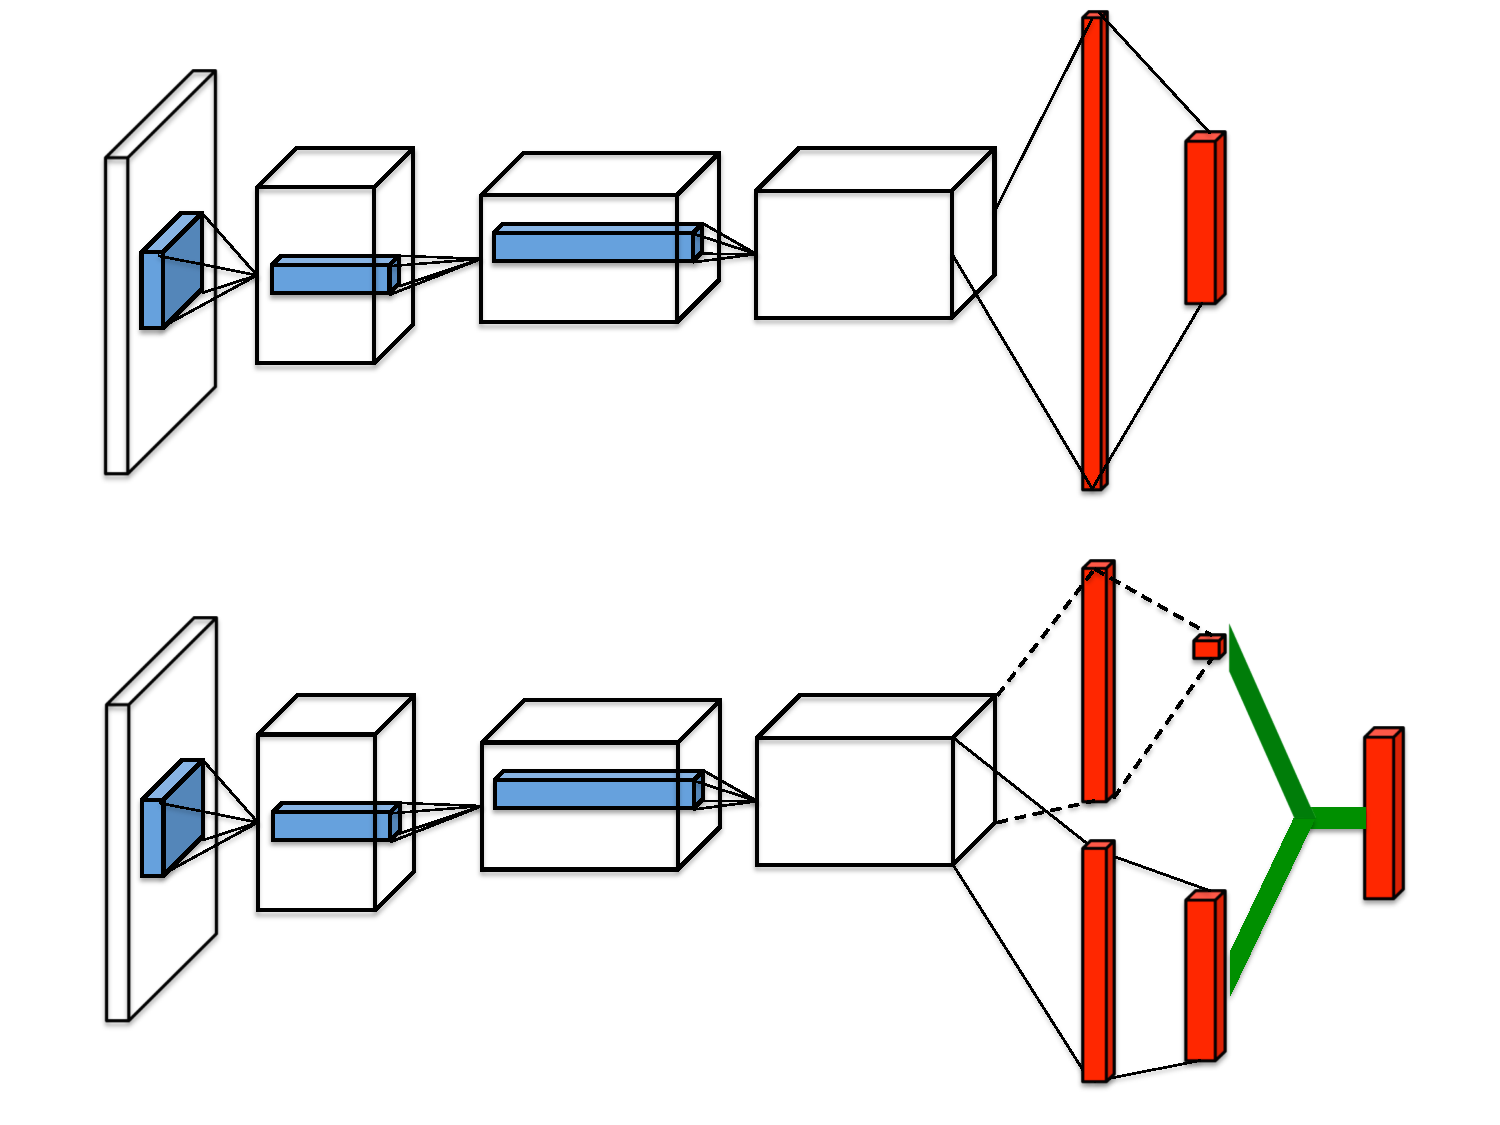
\includegraphics[width=0.95\linewidth]{fig/ddqn.pdf}
\caption[Dueling Network Architecture]{The dueling network architecture \cite{wang15_duelin_networ_archit_deep_reinf_learn} \label{fig-model-dueling}}
\end{figure}


Our agent uses the dueling DDQN algorithm with a standard neural network
architecture, similar to the one depicted in Figure \ref{fig-ann}. It consist of
four input nodes (number of states), three fully-connected hidden layers with
ReLU activation functions, and a linear output layer with two nodes (number of
actions). Further, an \(\epsilon\)-greedy policy with a linear decreasing
exploration rate was used. The RL agent was implemented with the neural networks
API Keras\footnote{\url{https://www.keras.io}}\textsuperscript{,}\,\footnote{\url{https://github.com/keras-rl/keras-rl}}, which is a high-level abstraction layer of TensorFlow.
TensorFlow is the de-facto standard for robust and scalable machine learning in
industry and research \cite{abadi16_tensor}. Further, we used the shared research
environment Google Colaboratory to train and evaluate the agent. It offers
free access to computing resources that are optimized for training machine
learning models.\footnote{Google Colaboratory (\url{https://colab.research.google.com}) provides a NVIDIA Tesla K80 GPU, with
2880 \(\times\) 2 CUDA cores and 12GB GDDR5 VRAM. Additionally, the environment is
equipped with a Intel(R) Xeon(R) CPU @ 2.30GHz (1 core, 2 threads), and 12GB
available memory. Google Colaboratory can be used up to 12 hours of consecutive
training time.

\clearpage}

\section{Results}
\label{sec:org94f029a}
The following chapter will cover the main results of this research. First, the
simulation environment is presented. Second, we examine the economic
sustainability of an integrated bidding strategy. Third, the RL approach that
aims to optimize the VPP portfolio is evaluated. In the last section, we will
perform sensitivity analyses on the limiting algorithmic factor, the prediction
accuracy, and a limiting physical factor, the charging infrastructure.

\subsection{Simulation Environment}
\label{sec:org24862d1}
As part of this research, we developed an event-based simulation platform called
\emph{FleetSim}. The platform allows researchers to develop and test out different
smart charging and bidding strategies in realistic environment based on
real-world data. In FleetSim, intelligent agents (called controllers) centrally
control the charging of an EV fleet, they are responsible to sufficiently charge
their vehicles to satisfy real mobility demand. At the same time, the agents can
create VPP of EVs, provide balancing services to the grid, and take part in
electricity trading. Trips are simulated on an individual level, for example,
not charging an individual EV at a particular point in time, can cause a whole
series of lost rentals, due to an insufficient amount of battery for the next
arriving customers. The agents are evaluated based on the profits of charging
the fleet cheaper than the industry tariff, the costs of losing rentals and the
imbalance they cause if they can not provide market commitments. Additionally,
FleetSim facilitates easy sensitivity analyses, adaption to future market
designs, and integration of novel data sets through its modular architecture and
expandable design (see Figure \ref{fig-fleetsim}). We consider FleetSim as a
research platform for sustainable and smart mobility similar to PowerTac
\cite{ketter16_multiagent_comp_gaming}. It builds on SimPy\footnote{\url{https://pypi.org/project/simpy/}}, a process-based
discrete-event simulation framework. FleetSim is available open source\footnote{\url{https://github.com/indyfree/fleetsim}} and
can be readily installed as a Python package.

\begin{figure}[hp]
\centering
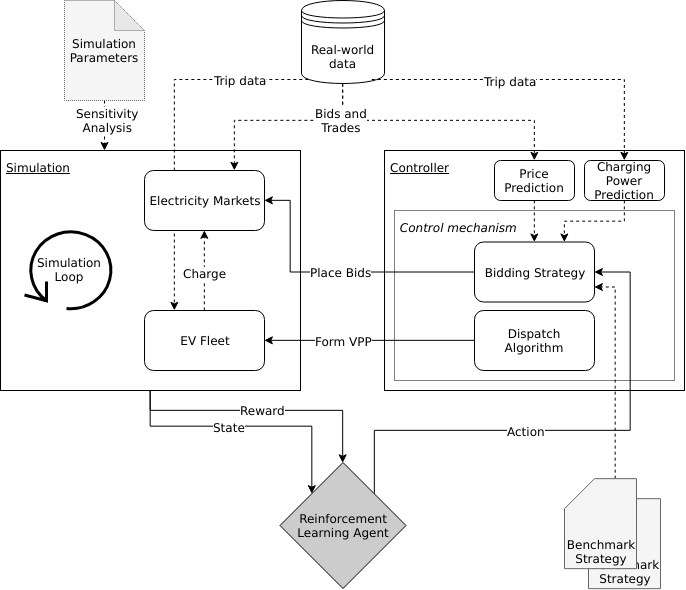
\includegraphics[width=1\linewidth]{fig/simulation-platform.png}
\caption[FleetSim Architecture]{Architecture of FleetSim \label{fig-fleetsim}}
\end{figure}

In order to simplify comparability and focus to real-world applicability of the
analysis, we set the same parameters for all conducted experiments (see Table
\ref{table-sim-params}). They are corresponding to the real Car2Go specifications
described in Chapter \ref{sec-data-car2go}. Further, we fixed the unknown
prediction accuracy of the fleets available charging power \(\fPhat{}\) to an
estimate of modern forecast algorithms performance. The impact of the
predictions uncertainty on the results will later be determined in a sensitivity
analysis.

\begin{table}[hp]
\caption[Simulation Parameters]{Simulation Parameters \label{table-sim-params}}
\centering
\begin{tabular}{lr}
\hline
\hline
Parameter & Value\\
\hline
EV battery capacity (\(\Omega\)) & 17.6 \(\kwh\)\\
EV charging power   (\(\gamma\)) & 3.6 \(\kw\)\\
EV range & 145 km\\
Industry electricity price  (\(p^{ind}\)) & 0.15\footnotemark \(\ekwh\)\\
EV rental tariff & 0.24\footnotemark \(\frac{\eur}{\text{min}}\)\\
EV long distance fee (\(>\text{200 km}\)) & 0.29\textsuperscript{\ref{orgdd4f310}} \(\frac{\eur}{\text{km}}\)\\
\hline
Prediction accuracy \(\fPhat{}\) week ahead & 70\%\\
Prediction accuracy \(\fPhat{}\) 30 min ahead & 90\%\\
\hline
\hline
\end{tabular}
\end{table}\footnotetext[12]{\label{orga3ba78a}Average prices of electricity for the industry with an annual consumption
of 500 MWh - 2000 MWh in Germany 2017 \cite{bmwi.19_prices_german}.}\footnotetext[13]{\label{orgdd4f310}Rental fees according to the Car2Go pricing scheme. See
\url{https://www.car2go.com/media/data/germany/legal-documents/de-de-pricing-information.pdf},
accessed 15\textsuperscript{th} March 2019.}

\subsection{Integrated Bidding Strategy}
\label{sec:orgc876434}
Research Question 1 examines whether a fleet operator can use a VPP portfolio of
EVs to profitably bid on multiple electricity markets. In Chapter
\ref{sec-model-mechanism}, we proposed a central control mechanism that charges
the fleet with an integrated bidding strategy. The following section evaluates
the results of the control mechanism in the simulation environment.

Table \ref{table-sim-stats} shows the descriptive statistics of the fleet
utilization during a simulation run, with data from June 1, 2016 to January
1, 2018. It can be observed that (a) the volatility of EVs parked at a charging
station is remarkably high (large standard deviation), and (b) the fraction of
EVs that can be utilized for VPP activities is diminishing low (3.55\%). It is
apparent that a high uncertainty and the low share of EVs that can possibly
generate profits are challenging the economic sustainability of our proposed
model. Figure \ref{fig-fleet-utilization} shows that despite a changing rental
behavior throughout the day (e.g., rush hour peaks between 7:00-9:00 and
17:00-19:00), the amount of EVs that can utilized for VPP activities is
comparably stable throughout the day.

\begin{figure}[h]
\centering
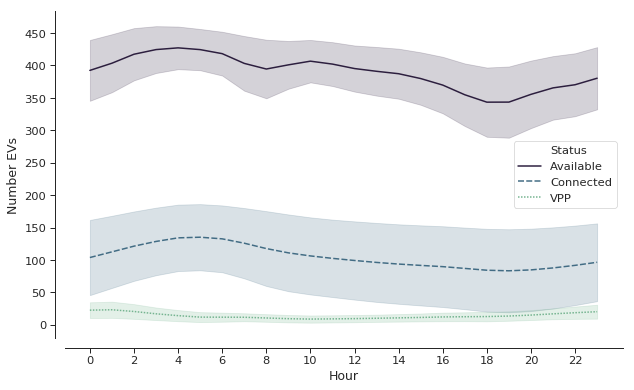
\includegraphics[width=1\linewidth]{fig/fleet-utilization.png}
\caption[Fleet Utilzation]{Daily fleet utilization (average, standard deviation) from June 1, 2016 to January 1, 2018. The blue error band is illustrating the large volatility in the amount of EVs that get parked at a charging station. The share of EVs that can be used as VPP is on average only 3.55\% of the fleet's size. Most of the EVs are either not connected to a charging station or are already fully charged. \label{fig-fleet-utilization}}
\end{figure}

\begin{table}[hp]
\caption[Fleet Statistics]{Fleet Statistics. \label{table-sim-stats}}
\centering
\begin{tabular}{lr}
\hline
\hline
Statistic & Value\\
\hline
Fleet size & 508\\
EVs available (min, max, \textbf{std}) & 389.64 (165, 496, \textbf{49.18})\\
EVs connected (min, max, \textbf{std}) & 61.23 (34, 290, \textbf{61.11})\\
VPP EVs (min, max, \textbf{std}) & 13.84 (0, 94, \textbf{9.01})\\
\hline
\hline
\end{tabular}
\end{table}

We defined several "naive" bidding strategies to evaluate and benchmark the
performance of our developed model. The strategies are naive in that sense that
they are assuming a fixed risk associated with bidding at a specific electricity
market. As opposed to the developed RL agent, they do not take information of
their environment into account and adjust the bidding quantities dynamically.
Instead, the controller discounts the predicted amount of available charging
power with a fixed risk factor \(\lambda\) (see \eqref{eq-model-pb} and
\eqref{eq-model-pi}). Naturally, the controller estimates a higher risk for
bidding on the balancing market week ahead than on the intraday market 30
minutes ahead. We defined following types of strategies:
\begin{enumerate}
\item Risk-averse (\(\lb{}\!=\!0.5\), \(\li{}\!=\!0.3\))

The controller avoids denying rentals and causing imbalances at all costs. In
order to not commit more charging power that it can provide, it places only
bids for conservative amounts of electricity on the markets. The risk-averse
strategies \emph{Balancing} and \emph{Intraday} are comparable to similar strategies
developed by
\textcite{kahlen17_fleet,kahlen18_elect_vehic_virtual_power_plant_dilem}.

\item Risk-seeking (\(\lb{}\!=\!0.2\), \(\li{}\!=\!0.0\))

The controller aims to maximize its profits by trading as much electricity on
the markets as possible. It strives to fully utilize the VPP and allocate a
high percentage of available EVS to charge from the markets. Due to the
rental uncertainty and a low estimated risk, the controller is prone to
offering more charging power to the markets that it can provide. This may
lead to lost rental costs or even imbalances.

\item Full information

The optimal strategy to solve the controlled charging problem. The controller
knows the bidding risks in advance and places the perfect bids on the
markets. In other words, it charges the maximal amount of electricity from
the markets without having to deny rentals or causing imbalances due to
prediction uncertainties.
\end{enumerate}

In Table \ref{table-profits}, the simulation results of all tested strategies are
listed. As expected, the developed integrated bidding strategies outperform
their single market counterparts. The controller is able to capitalize on the
most favorable market conditions and better utilizes the VPP by buying more
electricity from the markets than charging the EVs regularly. The integrated
strategies are resulting in 49\%-54\% more profits for the fleet than the single
market strategies.

A controller bidding according to the \emph{Integrated (risk-averse)} strategy, pays
on average \red{$0.10 \ekwh$  How much?} less for charging the fleet than other
risk-averse strategies. A controller with an \emph{Integrated (risk-seeking)}
strategy, is even more profitable, despite having to account for lost rental
profits. On the other side, the controller caused imbalances (highlighted red)
which lead to high (unknown) market penalties or even exclusion from bidding
activities. For this reason, imbalances need to be avoided, regardless of
potential profits from a higher VPP utilization. We expect that the proposed RL
agent learns a bidding strategy, which avoids imbalances while increasing
profits at the same time. The upper bound of the optimal strategy \emph{Integrated
(full information)}.

\red{Balancing power, stability}

{\captionsetup[table]{aboveskip=0.5cm}
\begin{sidewaystable}[hp]
\caption[Bidding strategy outcomes]{Outcomes of naive bidding strategies over a 1.5 year period. Integrated bidding strategies outperform single market strategies. \label{table-profits}}
\centering
\begin{tabular}{l|cccccc}
 & \thead{Balancing\\(risk-averse)} & \thead{Intraday\\(risk-averse)} & \thead{Integrated\\(risk-averse)} & \thead{Integrated\\(risk-seeking)} & \thead{Integrated\\(full information)}\\
\hline
\hline
VPP utilization (\%) & 39 & 47 & 62 & 81 & 71\\
Energy bought (MWh) & 803 & 985 & 1292 & 1681 & 1473\\
Energy charged regularly (MWh) & 1278 & 1096 & 789 & 400 & 608\\
Lost rental profits (1000 \eur) & 0 & 0 & 0 & 15.47 & 0\\
No. Lost rentals & 0 & 0 & 0 & 1237 & 0\\
Imbalances (MWh) & 0 & 0 & 0 & \textcolor{red}{1.01} & 0\\
Average electricity price (\(\ekwh\)) & - & - & - & - & -\\
Gross profit increase (1000 \eur) & 43.62 & 45.08 & \textbf{67.04} & \textbf{72.51} & 77.36\\
\hline
\hline
\end{tabular}
\end{sidewaystable}

}

\subsection{Reinforcement Learning Portfolio Optimization}
\label{sec:orgd24217c}
Research Question 2 investigates whether a RL agent can optimize the integrated
bidding strategy by dynamically adjusting the bidding quantities. The bidding
quantities \(\Pb{}, \Pi{}\) are based on the evaluated risk associated with
bidding on the individual electricity markets. In Chapter \ref{sec-model-rl}, we
introduced a RL approach that learns the risk factors \(\lb{}\), \(\li{}\) based on
its observed environment and received reward signals. In Appendix
\ref{app-rl-hyperparams}, the hyperparameters are presented which we used to train
the dueling DDQN algorithm and solving the controlled charging problem under
uncertainty. The values were determined manually through experimentation for the
best results. The speed of convergence was also used as a criterion, since the
training environment Google Colaboratory only allows up to 12 hours of computing
time.

Further, the imbalance costs \(\beta\) were set to an artificially high value to
incentivize the agent to learn to always avoid imbalances. Whenever the agents
takes an action that causes imbalances (i.e., bid too much electricity), it will
receive a highly negative reward signal, leading to a low estimated Q-value of
that chosen action in a specific state.

\begin{figure}[h]
\centering
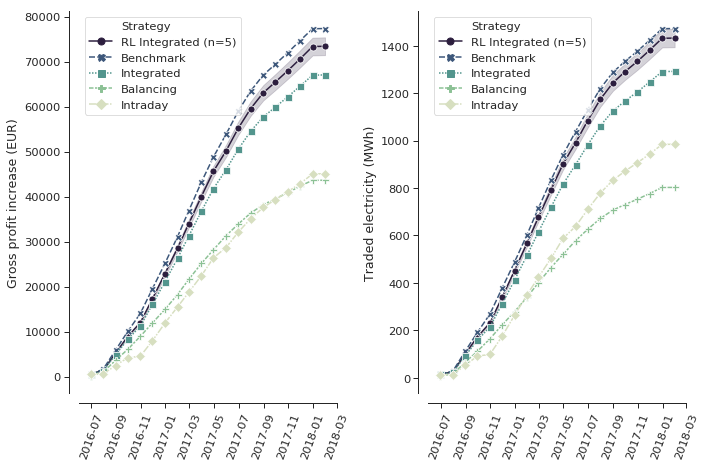
\includegraphics[width=1\linewidth]{fig/rl-results.png}
\caption[Comparison of gross profit results]{Comparison of gross profits and traded electricity between the proposed optimized integrated strategy and the other three naive charging strategies. The RL algorithm improves the achieved gross profit increase of the integrated bidding strategy on average by 12\% and accomplishes nearly optimal results when compared to the benchmark strategy. \label{fig-rl-profits}}
\end{figure}

In Figure \ref{fig-rl-profits}, the performance of the optimized integrated
bidding strategy is presented. The proposed RL algorithm increases the gross
profits of the fleet on average (n=5) by approximately 72-75\% when compared with
the naive single market strategies and by approximately 12\% when compared with
the naive integrated strategy. In none of the tested strategies the controller
procured more electricity from the market that it can charge. To reach the
optimal solution the gross profits would need to be increased by 3\% further.
Similarly, the RL algorithm increases the amount of electricity that the fleet
charges from the electricity markets while avoiding imbalance at the same time.
\red{Balancing power, renewables}

In another experiment, we evaluated the performance of the proposed RL algorithm
in comparison to other RL algorithms with a simpler architecture. In particular,
we were interested what impact modern advances in deep RL have on the ability to
quickly learn to improve the agents policy, while still achieving good results
after the whole training period. This question is especially relevant for the
case, when no prior training for the fleet controller is possible and the agent
has to quickly learn to avoid procuring more energy from the markets that it can
charge. Therefore, we removed the notion of imbalance costs and changed the
simulation setup to instantly stop the training episode when imbalances occur.
In this way, the agents learns to maximize its reward while circumventing
imbalances at all costs. The agent achieves a higher reward the longer it trades
electricity on the markets without committing to charge more electricity than it
can. We compared the DQN algorithm
\cite{mnih15_human_level_contr_throug_deep_reinf_learn} with the Double DQN
algorithm \cite{hasselt16_deep_reinf_learn_doubl_q_learn} with and without the
dueling architecture \cite{wang15_duelin_networ_archit_deep_reinf_learn}. In
Figure \ref{fig-rl-learning}, the average (n=5) learning performances of the
different RL approaches are displayed.

\begin{figure}[h]
\centering
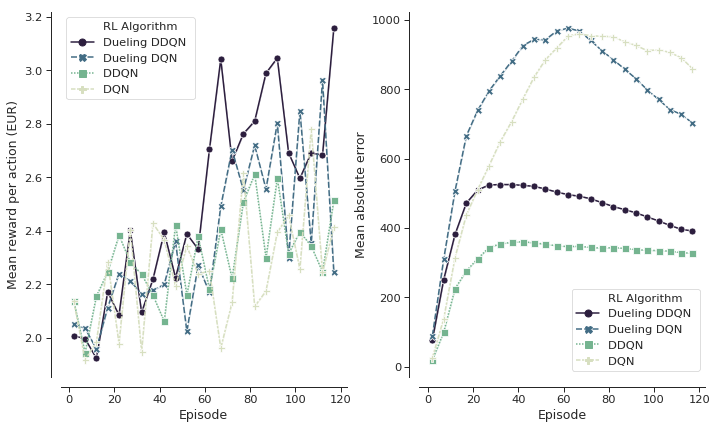
\includegraphics[width=1\linewidth]{fig/rl-learning.png}
\caption[Comparison of RL algorithm learning performance]{Comparison of the learning performance between the proposed RL algorithm and the other three simpler algorithms, averaged over 5 training attempts. Each training period is performed in 1.5 years simulation time with real world data. The dueling DDQN algorithm (dark blue line) learns faster, and achieves better end results than prior algorithms. \label{fig-rl-learning}}
\end{figure}

The experiment shows that the dueling DDQN algorithm learns the fastest and
shows a large increase in mean reward per action after roughly 60 episodes
(about 227 days of simulation time) of training. The dueling DDQN algorithm
shows the largest reward increase and highest reward per action after the whole
training period, which makes it the best algorithm to solve the charging
problem. Despite that it still has a larger mean absolute error than the DDQN
algorithm, indicating that it is more likely to cause imbalances with the
dueling architecture than without. None of the algorithms determined a policy
that never caused imbalances after training on the full 1.5 years of simulation
time (about one hour computing time). In other words, without prior training
with existing data the RL agent would need more than one and a half years to
learn to avoid imbalances. A possible explanation is the problem of learning
from long delayed rewards, first discussed by
\textcite{watkins89_learn_from_delay_rewar}. Long delayed rewards increase the
difficulty of RL problems, since the agent needs to connect occurring decision
outcomes to specific actions way back in the past. In the case of the presented
controlled fleet charging problem, this effect is especially pronounced because
a negative reward signal (caused imbalances) can occur up to 672 timesteps (one
week) after the agent decided on the bidding quantity for the balancing market,
whereas the reward signals from the intraday market occur almost immediately
after 2 timesteps (30 minutes).

In summary, both experiments show that our approach is able to learn a
profit-maximizing bidding strategy under varying circumstances, without using
any a priori information about the EV rental patterns. The proposed control
mechanism improves existing approaches and the RL agent can successfully
optimize the VPP portfolio strategy by estimating the risk that is associated
with bidding on the markets.

\subsection{Sensitivity Analysis}
\label{sec:orge3e6617}
The ability to accurately forecast the available fleet charging power plays an
important role in determining the optimal bidding quantity to submit to the
markets. If the fleet controller is certain about the number of connected EVs
that it can use for VPP activities in the future, it can aggressively trade the
available charging power on the markets, without being concerned about turning
away customers or facing the risk of not being able to charge the committed
amount. In our previous experiments, we assumed a fixed prediction accuracy that
we set to an estimate of what modern mobility demand forecasts capabilities. In
order to test the robustness of the results and their dependence on the
prediction accuracy, we conducted a sensitivity analysis. Therefore, we run five
simulation runs with the previously introduced RL approach but fixated the
prediction accuracy to increasing levels from 50\% to 100\% accurate forecasts, 7
days and 30 minutes ahead.

\begin{figure}[htbp]
\centering
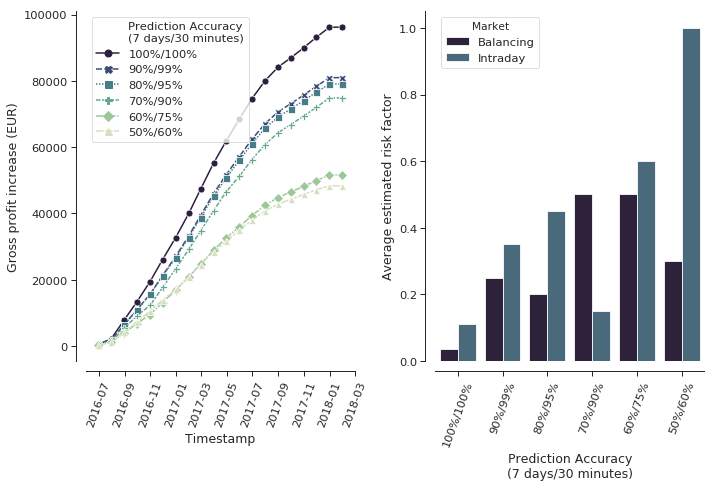
\includegraphics[width=1\linewidth]{fig/rl-accuracy.png}
\caption[Sensivity Analysis: Prediction Accuracy]{Sensivity Analysis: Prediction Accuracy \label{fig-sens-accuracy}}
\end{figure}

In Table \ref{fig-sens-accuracy} the results of the sensitivity analysis are
presented. The left plot shows the effect of the prediction accuracy on the
total gross profit increase, whereas the right plot shows the effect on the
learned risk factors of the RL agent. Intuitively the realized profit increases
with rising accuracy of the forecasts, while the estimated risk factors decrease
with more accurate forecasts. \red{Sentence to learned risk factors} Remarkably,
the magnitude of the effect on the profit increase is very prominent. After 1.5
years of simulation time, a RL agent that can rely on perfect predictions (100\%
accuracy) generates almost twice as much profit from trading electricity than
an agent that can only rely on predictions with 50\% and 60\% accuracy, 7 days and
30 minutes ahead respectively. It is striking that the prediction accuracy has a
larger effect \red{Quantitize!?} on the realized profit than the type of
bidding strategy or choice of RL algorithm, which we examined in the previous
chapters.

\clearpage

\section{Conclusion}
\label{sec:org86b0979}
Integrating volatile renewable energy sources into the electricity system
imposes challenges on the electricity grid. In order to ensure grid stability
and avoid blackouts, balancing power is needed to match electricity supply and
demand. Balancing power can be provided by VPPs that generate or consume energy
within a short period of time and offer these services on the electricity
markets \cite{pudjianto07_virtual_power_plant_system_integ}. EV fleet operators
can utilize idle vehicles to form VPPs and offer available EV battery capacity
as balancing power to the markets. The fleet can offer balancing services
directly via tender auctions on the balancing market or via continuous trades on
the intraday market, where participants procure or sell energy to self-balance
their portfolios \cite{pape16_are_fundam_enoug}. Both markets have complementary
properties in terms of price levels and lead times to delivery, which motivates the
creation of a VPP portfolio to profitably participate in both markets and extend
the business model of the fleet.

However, there are certain risks associated  with this business model extension.
EVs can only be allocated to a VPP portfolio if they are connected to a charging
station and have sufficient free battery capacity available, information which
is unknown to the fleet at the time of market commitment. This uncertainty makes
it difficult for fleet operators to estimate the size of the VPP and calculate
the optimal bidding quantities. Moreover, if fleet operators offer more
balancing power than they can provide, they face high imbalance penalties from
the markets. For a sustainable business model fleet operators also need to
balance VPP activities with their primary offering, customer mobility. Denying
customer rentals to ensure that the fleet can fulfill the market commitments,
results in opportunity costs of lost rentals that compromise the profitability
of the fleet.

In the following chapter, we will summarize the conducted research of this
thesis to address the aforementioned challenges. Furthermore, the contribution
of this work is outlined and the main results are presented and discussed.
Finally, we list specific limitations of this study and give insights on further
areas of research.
\subsection{Contribution}
\label{sec:org9c4d43a}
The core contributions of this thesis are the following: First, we
conceptualized a DSS for controlled EV charging under uncertainty. The DSS
constitutes the core of a business model extension for fleet operators to manage
a VPP portfolio of EV batteries. A controlled charging problem has been
mathematically formulated and a control mechanism introduced that aims solve the
proposed problem. Second, we developed an event-based simulation platform that
facilitates fleet management research with real-world data. We evaluated various
baseline bidding strategies within the simulation platform and tested out the
behavior of intelligent agents in the context of controlled EV charging. Third,
we proposed a novel integrated bidding strategy that offers balancing services
of a VPP portfolio to multiple electricity markets simultaneously. Instead of
submitting only conservative amounts of battery capacity to a single market,
like previous studies did
\cite{kahlen18_elect_vehic_virtual_power_plant_dilem,kahlen17_fleet}, our proposed
strategy aims to maximize profits by procuring electricity from the multiple
markets to the greatest extent possible without causing imbalances. Forth, we
proposed the usage of a RL agent that learns to optimize the composition of the
VPP portfolio and the associated risks of bidding on the markets. The agent
dynamically determines a risk factor, depending available and predicted fleet
and market information. Therefore, we formulated a MDP that is designed for
agents to work in previously unknown environments and uncertain conditions. The
RL agent is designed with the focus on real-world applicability and fast
convergence rates. Because we aimed for generalizability, we expect the proposed
approach to work in a variety of different settings, with different kinds of EVs
(e.g., electronic bikes) and independent of the geographical location of the
fleet.

We evaluated the proposed method with real-world carsharing data from Car2go in
Stuttgart and German electricity market data from June 2017 until January 2018.
The results show that the developed method improves existing approaches and
would increase the gross profits of the fleet by roughly \(78 000\; \eur\) over
the 1.5 year period. Since free float carsharing has inherently uncertain demand
patterns, better results are expected with other kinds of EV fleets. We found
that the integrated bidding strategy generates 49\%-54\% more profits, compared to
the naive benchmark strategies. Fleet controllers following the integrated
bidding strategy, can mitigate risks and increase profits by exploiting market
properties of both markets. Further, we showed that the proposed RL agent can
optimize the integrated bidding strategy under uncertainty by roughly 15\%,
almost \red{how much?} reaching the optimal solution with full information
available. The agent was able to successfully estimate the bidding risk, avoid
imbalances and keeping lost rentals to a minimum.
\red{Balancing power, stabilized the grid}
Additionally, we tested and compared the performance of
modern RL algorithms and found that recent advances in deep RL do improve the
robustness and convergence rates in real-world applications. Despite these
improvements, all RL approaches needed more than 1.5 years of simulation time to
learn to avoid imbalances penalties, which makes RL agents unsuitable to deploy
in unseen fleet environments without prior training data. A sensitivity analysis
of the prediction accuracy of the fleet balancing power showed that the accuracy
has large impact on the fleet profitability. If the controllers predictions are
very uncertain, the RL agent estimates high bidding risks and can only offer
conservative amounts of balancing power on the markets. Surprisingly, the effect
of prediction accuracy on the total gross profit increase is larger than the
choice of bidding strategy or RL algorithm architecture, which leaves room for
future research.



\begin{itemize}
\item Integrated bidding strategy exploit multiple markets properties
\item Online learning algorithm (difference? -- real data?)
\item Advantage over forecast like Kahlen: General, unseen, etc..
\end{itemize}


Impact on grid: Balancing power, mention balancing power.

Discuss:
\begin{itemize}
\item Compare to other studies!
\begin{itemize}
\item Fleet Charging
\begin{itemize}
\item No uncertainty
\item Only one market
\item No sensitivity on accuracy prediction (We found very important)
\end{itemize}
\item Other approaches (VPP, stochastic)
\cite{kahlen18_elect_vehic_virtual_power_plant_dilem} (no imbalance costs!)
\cite{vandael15_reinf_learn_heuris_ev_fleet}
\end{itemize}

\item Discuss results?
\begin{itemize}
\item Gross profits small - Mention before?
\item Policy
\item Investment
\item V2G?
\item Market Setup
\end{itemize}
\end{itemize}

\subsection{Limitations}
\label{sec:org75b7b3d}
\begin{itemize}
\item Model:
\begin{itemize}
\item Bidding Mechanism: one week ahead, always accepted
\item Policy \& Regulation: EVs not allowed to provide balancing power, minimum
bidding quantities 1MW.
\item Markets: Fleet is a price-taker, what about larger fleets? Simulate market influence
\item Deny rentals only in the same market period (More deny, less imbalance)
\end{itemize}
\item RL: See \cite{vazquez-canteli19_reinf_learn_deman_respon} conclusion for
limitations.
\begin{itemize}
\item Training time in real time. Generalization to other cities?
\end{itemize}
\end{itemize}
\subsection{Future Research}
\label{sec:org3b031f1}

\begin{itemize}
\item This result shows that leaving promising room for future research of highly
\end{itemize}
accurate mobility demand algorithms.
\begin{itemize}
\item Model:
\begin{itemize}
\item Investigate modern/current market design, that changed their bidding
mechanisms to to better integrate renewable energy generators.
\begin{itemize}
\item Daily/Day-ahead tenders with 4 hour market periods.
\end{itemize}

Mischpreisverfahren

i.e. daily w/ 4h slots. German "Mischpreisverfahren"
\end{itemize}
\item RL: Long-delayed rewards, different reward structure, memory based
\item Prediction Algorithms improvement, reference to sensitivity analysis
\end{itemize}

\clearpage
\appendix
\captionsetup[table]{list=no}
\captionsetup[figure]{list=no}


\section{Appendix: Data Tables \label{app-data-tables}}
\label{sec:orgb477d45}
\renewcommand\thetable{\thesection.\arabic{table}}
\setcounter{table}{0}

{\captionsetup[table]{aboveskip=0.5cm}
\begin{sidewaystable}[hp]
\caption{List of Trades of the EPEX Spot Intraday Continuous Market}
\centering
\begin{tabular}{c|cccccccc}
\hline
\hline
Execution time & ID & Unit Price & Quantity & Buyer Area & Seller Area & Product & Product Time & Delivery Date\\
\hline
2017-12-04 06:54:55 & 8031392 & 51.00 & 5500 & Amprion & Amprion & Quarter & 07:15 - 07:30 & 2017-12-04\\
2017-12-04 06:53:26 & 8031391 & 59.00 & 10000 & TenneT & TenneT & Quarter & 07:15 - 07:30 & 2017-12-04\\
2017-12-04 06:53:26 & 8031390 & 58.90 & 10000 & TenneT & TenneT & Quarter & 07:15 - 07:30 & 2017-12-04\\
2017-12-04 06:53:15 & 8031389 & 52.30 & 7000 & 50Hertz & 50Hertz & Quarter & 07:15 - 07:30 & 2017-12-04\\
2017-12-04 06:53:13 & 8031386 & 59.00 & 500 & TenneT & TenneT & Quarter & 07:15 - 07:30 & 2017-12-04\\
2017-12-04 06:53:13 & 8031387 & 51.00 & 3600 & Amprion & Amprion & Quarter & 07:15 - 07:30 & 2017-12-04\\
2017-12-04 06:53:13 & 8031388 & 52.00 & 1400 & Amprion & Amprion & Quarter & 07:15 - 07:30 & 2017-12-04\\
2017-12-04 06:53:02 & 8031385 & 58.90 & 11000 & TenneT & TenneT & Quarter & 07:15 - 07:30 & 2017-12-04\\
2017-12-04 06:52:38 & 8031380 & 60.00 & 10000 & Amprion & Amprion & Quarter & 07:15 - 07:30 & 2017-12-04\\
2017-12-04 06:52:38 & 8031381 & 57.50 & 8000 & Amprion & Amprion & Quarter & 07:15 - 07:30 & 2017-12-04\\
2017-12-04 06:52:38 & 8031382 & 58.00 & 2000 & Amprion & Amprion & Quarter & 07:15 - 07:30 & 2017-12-04\\
2017-12-04 06:52:38 & 8031383 & 58.90 & 4000 & TenneT & TenneT & Quarter & 07:15 - 07:30 & 2017-12-04\\
2017-12-04 06:52:38 & 8031384 & 60.00 & 4000 & Amprion & Amprion & Quarter & 07:15 - 07:30 & 2017-12-04\\
2017-12-04 06:52:27 & 8031379 & 52.30 & 8000 & 50Hertz & 50Hertz & Quarter & 07:15 - 07:30 & 2017-12-04\\
2017-12-04 06:51:33 & 8031378 & 66.00 & 5000 & TransnetBW & TransnetBW & Quarter & 07:15 - 07:30 & 2017-12-04\\
2017-12-04 06:51:28 & 8031377 & 54.00 & 8000 & Amprion & Amprion & Quarter & 07:15 - 07:30 & 2017-12-04\\
2017-12-04 06:51:24 & 8031376 & 54.00 & 7000 & TenneT & TenneT & Quarter & 07:15 - 07:30 & 2017-12-04\\
2017-12-04 06:49:34 & 8031375 & 51.00 & 4000 & TenneT & TenneT & Quarter & 07:15 - 07:30 & 2017-12-04\\
2017-12-04 06:49:26 & 8031374 & 54.00 & 5000 & 50Hertz & 50Hertz & Quarter & 07:15 - 07:30 & 2017-12-04\\
2017-12-04 06:49:23 & 8031373 & 55.10 & 8000 & 50Hertz & 50Hertz & Quarter & 07:15 - 07:30 & 2017-12-04\\
\hline
\hline
\end{tabular}
\end{sidewaystable}
}
\clearpage

\section{Appendix: Data Preprocessing \label{app-data-processing}}
\label{sec:org356e2ea}
The raw Car2Go dataset contained about 63 million data points (7.82 GB) and has
been processed to only contain about 1.25 thousand data points (100 MB), while
still compromising all necessary information. The following preprocessing steps
have been taken to prepare the data for further analysis:

\begin{enumerate}
\item Determine rental trips

Rental trips were inferred based on changing GPS coordinates between two data
points of the same EV (see Table \ref{table-car2go-raw}, 4\textsuperscript{th} to 5\textsuperscript{th} row).
Since the GPS accuracy of industry sensors is approximately 5 meters under
open sky, and worse near buildings, bridges, and trees \footnote{See \url{https://www.gps.gov/systems/gps/performance/accuracy}, accessed 23\textsuperscript{th} February 2019.
\clearpage}, measurement
errors occur. To reduce the number of falsely identified trips, a decreased
resolution of a 10-meter radius was calculated. Note that we hereby assume
that customers do not undertake trips, which begin and end at the same
location. In total, 1246040 customer rentals were determined.

\item Determine trip distances

The trip distances were inferred based on the difference in SoC level before
and after the rental and the average energy consumption per kilometer.
Although the real distance that can be covered with a certain amount of
energy depends on driving style and traffic situation, we are confident that
the deviation will be small, since all trips take place within the same urban
space.

\item Determine rental profits

The rental profits were inferred based on the trip duration and the estimated
trip distance. Car2Go has a minutely pricing scheme with an additional long
distance fee that applies when the customer drives more than a specified
range. The rental profits form an important piece of information for our
model since they determine the opportunity cost \(\rho\) the fleet controller
has to account for if it denies the rental in favor of VPP activities.

\item Clean data
\begin{itemize}
\item \emph{Service trips}: 3308 rental trips were removed that had a trip duration
longer than the maximum allowed rental time of two days. We assume that
these trips were \emph{service trips} undertaken by Car2Go. When the EVs
returned with a higher SoC (e.g., they have been charged at the car repair
shop), the previous trip had to be altered to end at a charging station to
ensure charging consistency.
\item \emph{Incorrectly charged EVs}: 52 EVs were removed that showed incorrect
charging behavior. These EVs reported a battery level increase of more than 20\%
between trips or during trips, while not being located at a charging station.
\end{itemize}
\end{enumerate}
\section{Appendix: DDQN Hyperparameters \label{app-rl-hyperparams}}
\label{sec:orgc1a4fae}
\setcounter{table}{0}
\begin{longtable}{lr}
\caption[Hyperparameters for the dueling network DDQN algorithm]{Hyperparameters for the dueling network DDQN algorithm.}
\\
\hline
\hline
Hyperparameter & Value\\
\hline
\endfirsthead
\multicolumn{2}{l}{Continued from previous page} \\
\hline

Hyperparameter & Value \\

\hline
\endhead
\hline\multicolumn{2}{r}{Continued on next page} \\
\endfoot
\endlastfoot
\hline
Target network update interval & 0.01\\
Optimizer & Adam \cite{kingma14_adam}\\
Batch size & 32\\
Learning rate & 10\textsuperscript{-3}\\
Replay buffer size & 10\textsuperscript{5}\\
Warm-up steps & 1000\\
Training steps & 10\textsuperscript{5}\\
Discount factor \(\gamma\) & 0.99\\
Reward normalization & r \(\in\) [-1, 1]\\
Gradient clipping & Gradient in [-1, 1] for output layer\\
Network architecture & See Appendix \ref{rl-network-def}\\
\hline
\(\epsilon\)-greedy annealing & Linear over 10\textsuperscript{5} steps\\
\(\epsilon\)-greedy minimum value & 0.1\\
\hline
\hline
\end{longtable}
\clearpage
\section{Appendix: DDQN Network Definition \label{rl-network-def}}
\label{sec:orgefb3dfe}
\newtcblisting{tcbpythoncode}[1][Python]{%
  colback         = yellow!5        ,
  colframe        = yellow!50!black ,
  listing only                      ,
  title           = #1              ,
  halign title    = right           ,
  fonttitle       = \bfseries       ,
  listing engine  = minted          ,
  minted language = python
}
\begin{tcbpythoncode}
from keras.models import Sequential
from keras.layers import Dense, Activation, Flatten

# Define sequential neural network
model = Sequential()
model.add(Flatten(nb_states))
model.add(Dense(16))
model.add(Activation("relu"))
model.add(Dense(16))
model.add(Activation("relu"))
model.add(Dense(16))
model.add(Activation("relu"))
model.add(Dense(nb_actions))
model.add(Activation("linear"))

# Print summary
model.summary()
\end{tcbpythoncode}

\newtcblisting{output-tobi}[1][Console output]{%
  colback         = white        ,
  colframe        = gray,
  listing only                      ,
  title           = #1              ,
  halign title    = left           ,
  fonttitle       = \bfseries       ,
  listing engine  = minted          ,
  minted language = python
}

\begin{output-tobi}
_________________________________________________________________
Layer (type)                 Output Shape              Param #
=================================================================
flatten_2 (Flatten)          (None, 1)                 0
_________________________________________________________________
dense_6 (Dense)              (None, 16)                32
_________________________________________________________________
activation_5 (Activation)    (None, 16)                0
_________________________________________________________________
dense_7 (Dense)              (None, 16)                272
_________________________________________________________________
activation_6 (Activation)    (None, 16)                0
_________________________________________________________________
dense_8 (Dense)              (None, 16)                272
_________________________________________________________________
activation_7 (Activation)    (None, 16)                0
_________________________________________________________________
dense_9 (Dense)              (None, 121)               2057
_________________________________________________________________
activation_8 (Activation)    (None, 121)               0
=================================================================
Total params: 2,633
Trainable params: 2,633
Non-trainable params: 0
\end{output-tobi}
\clearpage

\bibliography{bibliography/references}
\bibliographystyle{apacite}
\end{document}
